\documentclass[a4paper,12pt,twoside]{memoir}

% Castellano
\usepackage[spanish,es-tabla]{babel}
\selectlanguage{spanish}
\usepackage[utf8]{inputenc}
\usepackage[T1]{fontenc}
\usepackage{lmodern} % Scalable font
\usepackage{microtype}
\usepackage{placeins}

\RequirePackage{booktabs}
\RequirePackage[table]{xcolor}
\RequirePackage{xtab}
\RequirePackage{multirow}

% Links
\PassOptionsToPackage{hyphens}{url}\usepackage[colorlinks]{hyperref}
\hypersetup{
	allcolors = {red}
}

% Ecuaciones
\usepackage{amsmath}

% Rutas de fichero / paquete
\newcommand{\ruta}[1]{{\sffamily #1}}

% Párrafos
\nonzeroparskip

% Huérfanas y viudas
\widowpenalty100000
\clubpenalty100000

\let\tmp\oddsidemargin
\let\oddsidemargin\evensidemargin
\let\evensidemargin\tmp
\reversemarginpar

% Imágenes

% Comando para insertar una imagen en un lugar concreto.
% Los parámetros son:
% 1 --> Ruta absoluta/relativa de la figura
% 2 --> Texto a pie de figura
% 3 --> Tamaño en tanto por uno relativo al ancho de página
\usepackage{graphicx}
\usepackage{subcaption}
\newcommand{\imagen}[3]{
	\begin{figure}[!h]
		\centering
		\includegraphics[width=#3\textwidth]{#1}
		\caption{#2}\label{fig:#1}
	\end{figure}
	\FloatBarrier
}


\graphicspath{ {./img/} }
% Capítulos
\chapterstyle{bianchi}
\newcommand{\capitulo}[2]{
	\setcounter{chapter}{#1}
	\setcounter{section}{0}
	\setcounter{figure}{0}
	\setcounter{table}{0}
	\chapter*{#2}
	\addcontentsline{toc}{chapter}{#2}
	\markboth{#2}{#2}
}

% Apéndices
\renewcommand{\appendixname}{Apéndice}
\renewcommand*\cftappendixname{\appendixname}

\newcommand{\apendice}[1]{
	%\renewcommand{\thechapter}{A}
	\chapter{#1}
}

\renewcommand*\cftappendixname{\appendixname\ }

% Formato de portada

\makeatletter
\usepackage{xcolor}
\newcommand{\tutor}[1]{\def\@tutor{#1}}
\newcommand{\tutorb}[1]{\def\@tutorb{#1}}

\newcommand{\course}[1]{\def\@course{#1}}
\definecolor{cpardoBox}{HTML}{E6E6FF}
\def\maketitle{
  \null
  \thispagestyle{empty}
  % Cabecera ----------------
\begin{center}
  \noindent
\includegraphics[width=\textwidth]{cabeceraSalud}\vspace{1.5cm}%
\end{center}
  
  % Título proyecto y escudo salud ----------------
  \begin{center}
    \begin{minipage}[c][1.5cm][c]{.20\textwidth}
        
\includegraphics[width=\textwidth]{escudoSalud.pdf}
    \end{minipage}
  \end{center}
  
  \begin{center}
    \colorbox{cpardoBox}{%
        \begin{minipage}{.8\textwidth}
          \vspace{.5cm}\Large
          \begin{center}
          \textbf{TFG del Grado en Ingeniería de la Salud}\vspace{.6cm}\\
          \textbf{\LARGE\@title{}}
          \end{center}
          \vspace{.2cm}
        \end{minipage}
    }%
  \end{center}
  
    % Datos de alumno, curso y tutores ------------------
  \begin{center}%
  {%
    \noindent\LARGE
    Presentado por \@author{}\\ 
    en la Universidad de Burgos\\
    \vspace{0.5cm}
    \noindent\Large
    \@date{}\\
    \vspace{0.5cm}
    %Tutor: \@tutor{}\\ % comenta el que no corresponda
    Tutores: \@tutor{} -- \@tutorb{}\\
  }%
  \end{center}%
  \null
  \cleardoublepage
  }
\makeatother

\newcommand{\nombre}{Marina Sainz Bermejo}
\newcommand{\nombreTutor}{Daniel Sarabia Ortiz} 
\newcommand{\nombreTutorb}{Jesús Enrique Sierra García} 
\newcommand{\dni}{71798718D} 

% Datos de portada
\title{Modelado dinámico de la diabetes tipo I y estudio de técnicas de control de la glucosa}
\author{\nombre}
\tutor{\nombreTutor}
\tutorb{\nombreTutorb}
\date{\today}


\begin{document}

\maketitle


\newpage\null\thispagestyle{empty}\newpage

%%%%%%%%%%%%%%%%%%%%%%%%%%%%%%%%%%%%%%%%%%%%%%%%%%%%%%%%%%%%%%%%%%%%%%%%%%%%%%%%%%%%%%%%
\thispagestyle{empty}


\noindent
\includegraphics[width=\textwidth]{cabeceraSalud}\vspace{1cm}

\noindent D. \nombreTutor, profesor del departamento de Digitalización, área de Ingeniería de Sistemas y Automática.

\noindent Expone:

\noindent Que el alumno D. \nombre, con DNI \dni, ha realizado el Trabajo final de Grado en Ingeniería de la Salud titulado 'Modelado dinámico de la diabetes tipo I y estudio de técnicas de control de la glucosa'. 

\noindent Y que dicho trabajo ha sido realizado por el alumno bajo la dirección del que suscribe, en virtud de lo cual se autoriza su presentación y defensa.

\begin{center} %\large
En Burgos, {\large \today}
\end{center}

\vfill\vfill\vfill

% Author and supervisor
\begin{minipage}{0.45\textwidth}
\begin{flushleft} %\large
Vº. Bº. del Tutor:\\[2cm]
D. \nombreTutor
\end{flushleft}
\end{minipage}
\hfill
\begin{minipage}{0.45\textwidth}
\begin{flushleft} %\large
Vº. Bº. del Tutor:\\[2cm]
D. \nombreTutorb
\end{flushleft}
\end{minipage}
\hfill

\vfill

% para casos con solo un tutor comentar lo anterior
% y descomentar lo siguiente
%Vº. Bº. del Tutor:\\[2cm]
%D. nombre tutor


\newpage\null\thispagestyle{empty}\newpage




\frontmatter

% Abstract en castellano
\renewcommand*\abstractname{Resumen}
\begin{abstract}
La combinación de la ingeniería y la biología, respaldada por la medicina, se presenta como una de las fronteras más prometedoras de la ciencia para el desarrollo de nuevas soluciones tecnológicas que supongan aumentos en la calidad de vida de pacientes con alguna patología.

La Diabetes Mellitus se consolida como uno de los mayores problemas de salud a nivel mundial, y los últimos datos recogen una prevalencia del 9.3 \% para la población entre 20 y 79 años. Es por ello por lo que el avance en el estudio del funcionamiento de los mecanismos que regulan la glucosa y la insulina es crucial para el surgimiento de nuevos dispositivos médicos que permitan avanzar hacia nuevas terapias y tratamientos de la diabetes. Este estudio comienza por el modelado del comportamiento glucémico en base a ecuaciones y relaciones matemáticas, que posteriormente puedan implementarse en sistemas de control para sustituir variables, como la administración de insulina externa en el organismo de forma manual, y que pueden verse condicionadas por otras variables existentes en la vida real. 

Se pretenden reflejar estas cuestiones en este análisis del comportamiento de la glucosa e insulina basado en razonamientos matemáticos, y comprobar si su estimación es similar funciomiento del organismo.

\end{abstract}

\renewcommand*\abstractname{Descriptores}
\begin{abstract}
Insulina, glucosa, sistema glucorregulatorio, diabetes mellitus, sistemas de control, modelos matemáticos, perturbaciones, simulación, control automático de la glucosa.
\end{abstract}

\clearpage

% Abstract en inglés
\renewcommand*\abstractname{Abstract}
\begin{abstract}
The combination of engineering and biology, supported by medicine, emerges as one of the most promising frontiers in science for the development of new technological solutions that lead to improvements in the quality of life of patients with any pathology.

Diabetes Mellitus is consolidated as one of the biggest public health problems worldwide, with recent data showing a prevalence of 9.3\% for the population aged between 20 and 79 years old. This is why progress in studying mechanisms regulating glucose and insulin is crucial for the emergence of new medical devices that allow advancements towards new therapies and treatments for diabetes. This study begins by modeling glycemic behavior based on equations and mathematical relationships, which can subsequently be implemented in control systems to replace variables such as manual administration of external insulin , and which may be influenced by real-life variables.

The aim is to reflect these issues in this analysis of the behavior of glucose and insulin based on mathematical reasoning, and to verify if their estimation is similar to the functioning of the organism.

\end{abstract}

\renewcommand*\abstractname{Keywords}
\begin{abstract}
Insuline, glucose, glucorregulatory system, mellitus diabetes, control systems, mathematical models, disturbances, simulation, authomatic glucose control.
\end{abstract}

\clearpage

% Indices
\tableofcontents

\clearpage

\listoffigures

\clearpage

\listoftables
\clearpage


\mainmatter
\capitulo{1}{Introducción}


La interacción entre la glucosa y la insulina en el organismo es un mecanismo biológico complejo cuyo correcto funcionamiento es fundamental para el bienestar y la vida de la sociedad. Alteraciones en esta interacción pueden desencadenar grandes riesgos, como es el caso de las patologías cardiovasculares o renales. Especial relevancia cobra en este estudio la enfermedad de la Diabetes Mellitus, caracterizada por la ausencia o falta de insulina en el cuerpo, que desencadena altos niveles glucémicos que suponen significativos riesgos para la salud.

En este proyecto se llevará a cabo un análisis del sistema glucorregulatorio, adecuado y alterado, a partir de modelos matemáticos que han ido surgiendo en las últimas décadas, que tratan de reflejar el comportamiento de las variables de la forma más próxima posible a la realidad. Además, en base a estos modelos es posible simular dinámicas de la glucosa ante entradas al sistema, como la administración de insulina exógena, así como estudiar el efecto de algunas perturbaciones como la ingesta o el ejercicio físico.

El avance en el conocimiento sobre estos mecanismos es clave para el desarrollo de dispositivos médicos que puedan contrarrestar los efectos nocivos en caso de haberlos, o bien para la mejora de la calidad de vida de los pacientes. Los sistemas de monitorización de glucosa, o sistemas más sofisticados, como el páncreas artificial, suponen mejoras revolucionarias e innovadoras que se traducen en grandes resultados para el tratamiento de la Diabetes Mellitus, por lo que también se ha considerado la inclusión de sencillos sistemas de control en el proyecto.

La gran parte de las simulaciones y experimentos llevados a cabo se encuentran en el apartado de resultados, mientras que las secciones Conceptos Teóricos y Metodología reúnen la información necesaria para obtenerlas. Es resto de la información relevante, para finalizar, está ubicada en el anexo.





\capitulo{2}{Objetivos}

Este trabajo surge de la inquietud en cuanto a la comprensión de los mecanismos biológicos y el desarrollo de estrategias y planes de control que aparecen para resolver los fallos de estos mecanismos. La complejidad de estas relaciones hace que sea necesario un alto conocimiento y precisión sobre ellas, especialmente en estos casos, en los que está involucrado el funcionamiento del propio cuerpo humano, y donde los riesgos pueden ser altamente perjudiciales, como es el caso de la Diabetes Mellitus.

\section{Objetivos del proyecto}

\begin{enumerate}
    \item Estudio del comportamiento del organismo, analizando la interacción de la glucosa e insulina en base al modelado matemático. Estos modelos cuentan con parámetros que reflejan interacciones de la glucosa, por lo que el análisis de su variación también se consolida como subobjetivo de este apartado.
    \item Estudio del comportamiento alterado del organismo, reflejado en la diabetes mellitus, y sus consecuencias en el sistema glucorregulatorio. Mediante un modelo modificado, analizar el efecto de las diferentes perturbaciones y de entradas, donde cobra especial relevancia la administración de insulina exógena para retornar a unas condiciones óptimas. La interacción entre estas variables se recoge como subobjetivo.
    \item Estudio de efecto de los sistemas de control glucémico en el organismo mediante el diseño de reguladores sencillos. Estas estrategias son la base para la implementación futura de sistemas regulatorios más complejos, como es el páncreas artificial. En este proyecto se emplea un regulador PID.
\end{enumerate}

\section{Objetivos personales}

\begin{enumerate}
    \item Profundizar en la comprensión del comportamiento de la glucosa e insulina, así como estudiar las variables que pueden influir en él.
    \item Iniciar el proceso de aprendizaje en el campo de la ingeniería de control, aplicando conocimientos matemáticos para establecer relaciones entre variables, y representarlas mediante simulaciones.
    \item Adquisición y dominio de LaTex como sistema de composición de texto para la creación de documentos técnicos.
    \item Comenzar este estudio que pueda ser empleado por otras personas en un futuro para el desarrollo de sistemas de control más sofisticados, o bien de modelos matemáticos innovadores.
\end{enumerate}



\capitulo{3}{Conceptos teóricos}


Se detallan a continuación los conceptos relevantes que se han considerado necesarios a incluir en esta sección.

\section{Glucosa e insulina}

\subsection{La glucosa}

La glucosa es un carbohidrato con fórmula empírica $ C_6H_{12}O_6$ que pertenece al grupo de las aldohexosas, pues contiene 6 átomos de carbono y presenta una aldosa.  Su grupo carbonilo se encuentra en el carbono 1 de la cadena carbonada.
Puede encontrarse de forma libre o combinada, y es el compuesto orgánico más abundante en la naturaleza. Su importancia radica en ser la principal fuente de energía de las células, realizando funciones como la oxidación catabólica. Además, es el componente principal de polímeros de gran importancia estructural como la celulosa, así como de polímeros de almacenamiento energético como el almidón o el glucógeno.


A nivel estructural, presenta más de una configuración, visible en la Figura \ref{fig:formula_glucosa} y obtenida de \cite{murray2007bioquimica}. Su forma lineal se compone de una cadena recta (aldohexosa), tal y como se ha definido al comienzo de la sección por su fórmula empírica. Además, puede encontrarse de forma cíclica, mediante un hemiacetal formado por reacción entre el grupo aldehído y el grupo hidroxilo. Esta configuración es favorecida en el aspecto termodinámico, y se dibuja mediante la proyección de Haworth resultando una estructura en anillo, de seis miembros, con los grupos hidroxilo situados por arriba o por debajo del plano.

\begin{figure}[h]
    \centering
    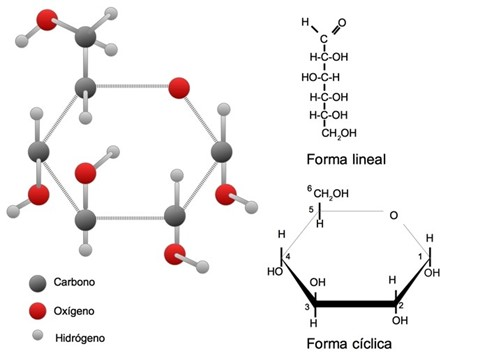
\includegraphics[width=0.7\textwidth]{img/imagen_formula_glucosa.jpg}
    \caption{Configuraciones de la glucosa.}
    \label{fig:formula_glucosa}
    \vspace{0.5cm} % Ajusta el espacio vertical entre la imagen y el texto
\end{figure}

La glucosa es el carbohidrato más simple, lo que lo convierte en un monosacárido e implica la presencia de azúcar. Sin embargo, otros monosacáridos también contienen azúcar, como la ribosa, la galactosa o la fructosa, con la que comparte fórmula, y respecto a la que se diferencia por la posición relativa de sus grupos -OH y O=.  
Presenta dos formas, la D- Glucosa y la L- Glucosa. La D-(+)-glucosa es uno de los compuestos más importantes para los seres vivos, incluyendo a seres humanos.
La glucosa en sangre es el principal azúcar de la sangre, y es la principal fuente de energía del cuerpo humano. Se obtiene de la ingesta de alimentos, y cuando estos se procesan, el azúcar pasa al torrente sanguíneo, por donde circula libre, y se almacena en forma de glucógeno. Entre sus funciones, destacan dos:

\begin{enumerate}
    \item[-] Obtención de energía, mediante su transformación a adenosín trifosfato (ATP) dentro de las células.
    \item[-] Reserva de energía, si el cuerpo no necesita su energía de forma inmediata, se almacena en forma de glucógeno en hígado y músculos.
\end{enumerate}

Los niveles de azúcar en sangre se encuentran dentro de unos rangos que garantizan el correcto funcionamiento del organismo. Los rangos infereriores suelen venir delimitados por la glucosa basal, que es el nivel de glucosa en ayunas, y cantidades muy inferiores a ella comprometen la estabilidad del organismo, causando hipoglucemia. El efecto contrario se denomina hiperglucemia. Estos niveles se regulan mediante una hormona denominada insulina. Además, esta hormona participa en el transporte de glucosa desde el torrente sanguíneo a las células, donde se utiliza la glucosa como energía.


\subsection{La insulina}

La insulina humana es una hormona de naturaleza proteína sintetizada en las células beta de los islotes de Langerhans del páncreas. Fue descubierta en 1921 y es secretada en respuesta a niveles elevados de glucosa, así como ante algunas hormonas peptídicas como el glucagón o la secretina.

Es una proteína globular muy conservada compuesta por 51 aminoácidos en su forma activa, como se muestra en la Figura \ref{fig:insulina_quimica} \footnote{Obtenido de \cite{insulina_website}}. En su centro proteico se encuentran los aminoácidos no polares, formando un núcleo hidrofóbico, mientras que los aminoácidos polares y cargados se sitúan alrededor del núcleo. Estos se distribuyen en 2 cadenas, A y B, de 21 y 30 aminoácidos respectivamente. Ambas cadenas interaccionan mediante puentes disulfuro.

\begin{figure}[h]
    \centering
    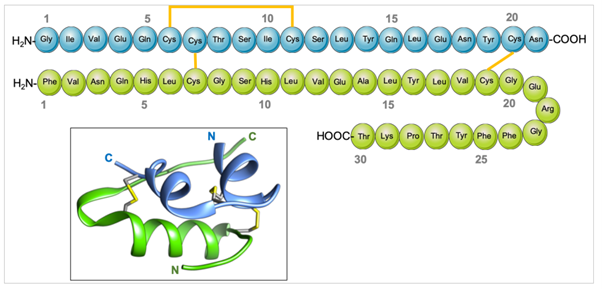
\includegraphics[width=0.7\textwidth]{img/imagen_insulina.png}
    \caption{Disposición de los aminoácidos de la insulina.}
    \label{fig:insulina_quimica}
\end{figure}

Las células del organismo, sin embargo, tienen dificultades para hacer que las proteínas se plieguen de forma correcta en estructuras estables. Como solución, se sintetiza una proteína más grande llamada proinsulina, en la Figura \ref{fig:proinsulina}.

El ARN mensajero de la insulina se traduce como un precursor de una cadena polipeptídica llamada preproinsulina, compuesta por 110 aminoácidos. Esta cadena, tras eliminarse su péptido señal durante su inserción en el retículo endoplasmático, da lugar a la proinsulina. Cuenta con 87 residuos y se modifica en el Aparato de Golgi. De él salen las vesículas secretoras con la hormona activa, la insulina.
A nivel estructural, la proinsulina presenta 3 dominios: una cadena de la amino terminal de la cadena B, con una alfa hélice;una cadena carboxi- terminal A con dos alfas hélices, y un péptido que conecta ambas conocido como péptido C.


\begin{figure}[h]
    \centering
    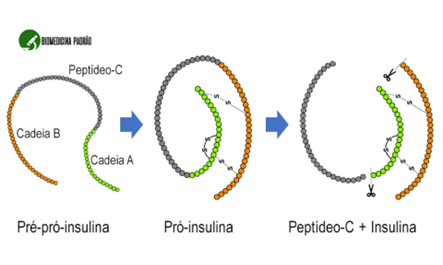
\includegraphics[width=0.7\textwidth]{img/imagen_proinsulina.png}
    \caption{Síntesis de insulina mediante proinsulina y el péptido C.}
    \label{fig:proinsulina}
\end{figure}

Por tanto, la insulina se sintetiza como preproinsulina. Esta molécula está formada por una sola cadena polipeptídica, que posteriormente y en diversas partes de la célula, sufre varios procesamientos para obtener finalmente la insulina activa.

Entre las funciones de la insulina, destacan dos. Por una parte, disminuye el nivel de glucosa sanguínea, como se ha comentado, favoreciendo la conversion de glucosa en glucógeno en los hepatocitos y miocitos siempre y cuando la glucosa se encuentre elevada. Por la otra parte, estimula la captación de glucosa en varios tipos de células, así como el almacenamiento y consumo de ésta en numerosos tejidos del cuerpo, y especialmente en músculos, tejido adiposo e hígado. Mientras que en el músculo incrementa el transporte de glucosa hacia el interior de las células musculares (que se consumirá para obtener energía en forma de ATP), en el hígado la insulina facilita la entrada de glucosa en células hepáticas, evita la liberación de glucosa a la sangre y promueve la síntesis de glucógeno. Así, en el tejido adiposo la insulina promueve, de forma indirecta, el depósito de grasas en forma de triglicéridos.
La acumulación de glucógeno en el hígado y de grasas en el tejido adiposo permite que el cuerpo tenga reservas de energía que poco a poco consumen durante el tiempo de ayunas para mantener una glucemia constante. Una vez que el organismo vuelve a estos valores normales de glucosa, se elimina la señal que provocó la síntesis de insulina, y esta deja de secretarse. La insulina también tiene, al igual que la glucosa, un valor basal, que delimita el rango inferior del comportamiento óptimo del organismo. Por debajo de este valor, se generan grandes riesgos para el metabolismo y funcionamiento celular adecuado.

\subsubsection{Insulina activa y concentración de insulina en sangre}

En este análisis se diferencian dos tipos de insulina:
\begin{enumerate}
    \item[-] \textit{Insulina}, se refiere a la cantidad total de insulina presente en el torrente sanguíneo en un momento dado. Puede medirse directamente mediante análisis de sangre, y representa tanto la insulina activa como cualquier otra forma de insulina presente en la sangre, ya sea unida a proteínas transportadoras, en forma de precursor inactivo o en cualquier otra forma.
    es la forma de la hormona que se secreta inicialmente por las células beta del páncreas en respuesta a un aumento en los niveles de glucosa en sangre. La insulina se secreta en su forma precursora, conocida como proinsulina, que luego se procesa para convertirse en insulina activa y péptido C gracias a una enzima específica llamada convertasa de prohormona (PC), que escinde el péptido C de la proinsulina.
    \item[-] \textit{Insulina activa}, se refiere específicamente a la fracción de insulina que está disponible para unirse a los receptores de insulina en los tejidos periféricos y ejercer su efecto biológico. Es la forma de insulina que ha sido procesada a partir de proinsulina, forma precursora de la insulina. 
\end{enumerate}


\section{Sistema glucorregulatorio}

Se denomina sistema glucorregulatorio al conjunto de mecanismos y procesos fisiológicos que el cuerpo utiliza para mantener los niveles de glucosa en la sangre dentro de un rango adecuado y saludable. Este sistema es crucial para el funcionamiento normal del organismo, ya que la glucosa es la fuente primaria de energía para las células; y se compone tanto de órganos como de hormonas.

\subsection{Actores principales en la glucorregulación}

El páncreas es el órgano principal en la regulación de la glucosa sanguínea. Contiene unas células especializadas llamadas células alfa y beta, situadas en los islotes de Langerhans (Figura \ref{fig:islotes} 
 \footnote{Obtenido de \cite{britannica_islets}}). Estas células secretan hormonas, la insulina y el glucagón, que están directamente implicadas en la variación de los niveles de glucosa en el organismo. 
\begin{figure}[h]
    \centering
    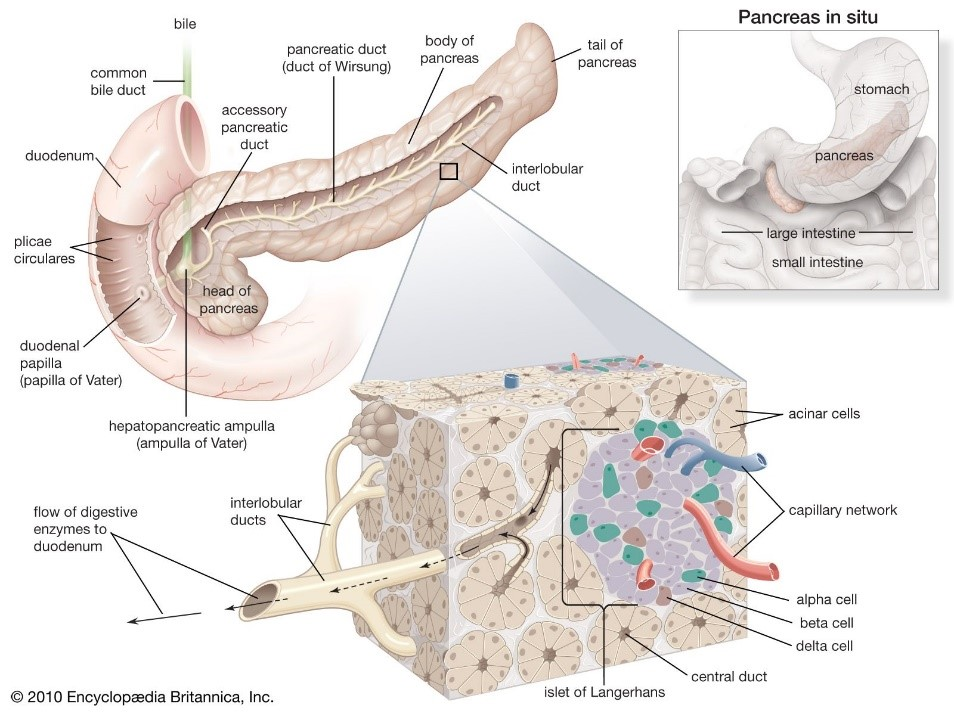
\includegraphics[width=0.8\textwidth]{img/imagen_islotes_langerhans.jpg}
    \caption{Islotes de Langerhans del páncreas y células beta y alfa.}
    \label{fig:islotes}
\end{figure}

Por su parte, el hígado almacena la glucosa en forma de glucógeno, y la libera cuando es necesario (ver Figura \ref{fig:basico_glucorregulatorio} \footnote{Obtenido de \cite{labster_glucose}}). También funcionan como depósito de almacenamiento de glucosa el músculo y tejido adiposo. El sistema nervioso central participa en la regulación de la glucosa mediante señales hormonales y nerviosas.
A nivel hormonal, son dos las hormonas principales del sistema glucorregulatorio. Por una parte, la insulina, como ya se ha comentado, es liberada por las células beta del páncreas cuando los niveles de glucosa en sangre son elevados. Facilita la entrada de glucosa a las células, especialmente en el hígado, músculos y tejido adiposo, para ser utilizada como energía o almacenada como glucógeno. Además, inhibe la producción de glucosa por el hígado (gluconeogénesis) , estimula la síntesis de glucógeno (glucogénesis) y facilita la conversión de glucosa en ácidos grasos para su almacenamiento.

La regulación del metabolismo de la glucosa por la insulina depende de un equilibrio muy delicado con otra hormona “hermana”, el glucagón, que se libera cuando los niveles de glucosa en sangre son bajos, generalmente durante la noche y entre las comidas, estimulando la conversión de glucógeno en glucosa en el hígado (gluconeogénesis), e inhibiendo la síntesis de glucógeno. 

Otras hormonas relevantes implicadas en el control de los niveles de glucosa en sangre son:
\begin{enumerate}
    \item[-] La adrenalina o epinefrina, producida por las glándulas suprarrenales, aumenta rápidamente los niveles de glucosa en respuesta al estrés. Actúa directamente sobre el hígado para promover la producción de azúcar, y promueve la descomposición y liberación de los nutrientes de la grasa que viajan hacia el hígado y que se convierten en azúcar y cetonas.
    \item[-] El cortisol es una hormona esteroide también secretada por la glándula suprarrenal que asimismo aumenta los niveles de glucosa en respuesta al estrés prolongado. En circunstancias normales, el cortisol compensa la acción de la insulina, pero bajo condiciones de estrés los niveles de cortisol se vuelven elevados y se adquiere insulino - resistencia. Bajo esta condición, las células del cuerpo no responden correctamente a la insulina, por lo que se necesita mayor cantidad de esta para lograr el mismo efecto de reducción de glucosa en sangre.
    \item[-] La hormona de crecimiento se libera desde la glándula pituitaria, en el cerebro, y compensa el efecto de la insulina sobre las células grasas y los músculos. Altos niveles de hormona de crecimiento provocan resistencia a la acción de la insulina.
    \item[-] Otras hormonas como las incretinas GLP-1 y GIP se producen en las células del intestino y potencian la secreción de insulina tras la ingesta, así como la amilina, cuyo efecto es muy similar.
\end{enumerate}
Pese a que esta hormonas quedan fuera del estudio presente, sería interesante comprender su funcionamiento en otros futuros análisis.

\subsection{Funcionamiento del sistema glucorregulatorio}
El sistema se rige por la variación de los niveles de glucosa en el organismo. 
Después de una comida, ver Figura \ref{fig:basico_glucorregulatorio} \footnote{Obtenido de \cite{velasquez2013modelado}.}, los niveles de glucosa se ven aumentados, lo que estimula a las células beta del páncreas a liberar insulina. Así, la glucosa de los alimentos se absorbe y llega a la sangre. La insulina la transporta a las células, donde se utiliza para ser almacenada en forma de glucógeno, ácidos grasos y aminoácidos. Como resultado, los niveles de glucosa en sangre disminuyen a niveles normales. Entre comidas, los niveles de glucosa en sangre comienzan a caer. Esta disminución estimula a las células alfa del páncreas a liberar glucagón. El glucagón actúa principalmente en el hígado, donde estimula la descomposición del glucógeno en glucosa, lo que aumenta los niveles de glucosa en sangre a niveles normales.

\begin{figure}[h]
    \centering
    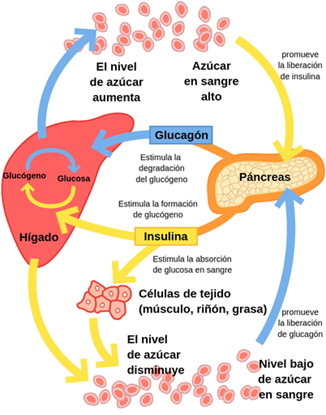
\includegraphics[width=0.5\textwidth]{img/imagen_funcionamiento_basico_glucosa.png}
    \caption{Funcionamiento básico de la regulación glucosa- insulina en el organismo.}
    \label{fig:basico_glucorregulatorio}
\end{figure}

Durante el ejercicio, la demanda de energía en los músculos aumenta, lo que provoca un mayor uso de glucosa. En respuesta, las glándulas suprarrenales liberan adrenalina, que estimula la liberación de glucosa y ácidos grasos para proporcionar energía rápida. Además, la adrenalina inhibe la liberación de insulina y estimula la liberación de glucagón, asegurando que haya suficiente glucosa disponible para satisfacer las necesidades energéticas del cuerpo.

\subsection{Alteraciones del sistema glucorregulatorio}

El equilibrio preciso y dinámico de los mecanismos que regulan la glucosa es esencial para la homeostasis del organismo y para la prevención de enfermedades relacionadas.
Las alteraciones en este sistema pueden ocurrir a varios niveles, que se dividirán en 4: alteraciones en la secreción de insulina, alteraciones en la acción de la insulina, alteraciones en la liberación y producción de glucosa, y alteraciones en la liberación de hormonas contrarreguladoras. Nos centraremos en las dos primeras.

Las alteraciones en la secreción de insulina comprenden la hiperinsulinemia y la hiperinsulinemia. La hiperinsulinemia se caracteriza por un aumento anormal de la secreción de insulina y puede ser una respuesta compensatoria a la resistencia a la insulina que se da en ocasiones. Como consecuencia, las células beta del páncreas deben producir más insulina y puede contribuir al desarrollo de diabetes tipo 2. La hipoinsulinemia produce, al contrario que la anterior, cantidades insuficientes de insulina. Esto da lugar a niveles elevados de glucosa en sangre, y puede ser causada por daño o fallo progresivo de las células beta del páncreas.

Respecto a las alteraciones en la acción de la insulina, destacan dos. La resistencia a la insulina, por una parte, implica que las células no respondan adecuadamente a ella. Por tanto, los niveles de glucosa se mantienen elevados y el páncreas es obligado a producir más insulina, lo que se vuelve perjudicial. Se asocia esta alteración a factores genéticos, obesidad, sedentarismo y dietas poco saludables. Por otra parte, pueden ocurrir defectos en la señalización de la insulina, como anomalías en receptores o en la cascada de señalización entre la insulina y su receptor, lo que contribuye a valores altos de glucosa.


\subsubsection{Patologías}
Existen consecuencias a largo plazo para los niveles de glucosa no regulados. Puede ocasionar una diversidad de condiciones, que incluyen neuropatía, enfermedad cardiaca, ceguera, infecciones de la piel, o el coma.
La alteración del sistema glucorregulatorio más conocida es la Diabetes Mellitus, y se caracteriza por una deficiencia en la producción o respuesta de insulina. Pese a ser conocida por la presencia de una glucemia elevada, puede aparecer en otras enfermedades como la feocromocitoma, las enfermedades renales, el hipertiroidismo, el glucagonoma, la pancreatitis aguda, el síndrome de Cushing o los tumores de páncreas.
En cambio, puede aparecer la glucemia disminuida en casos como: dietas con defecto en el aporte de glucosa, enfermedades hepáticas, enfermedad de Addison, exceso de insulina en diabéticos, hipopituitarismo, hipotiroidismo o insulinoma.
Si el cuerpo no produce suficiente insulina, puede ocasionar la liberación de ácidos grasos libres de las reservas de grasa. Esto puede ocasionar una condición llamada cetoacidosis. Las cetonas (residuos creados cuando el hígado descompone la grasa) pueden ser tóxicas en grandes cantidades.

\subsubsection{Hipoglucemia}
La hipoglucemia implica un bajo nivel de glucosa en sangre, frecuentemente por debajo de 70 mg/dL, aunque el valor puede variar para cada persona.
Los síntomas de estos bajos niveles tienden a aparecer rápidamente, y pueden incluir mareos, hambre, sudoración, irritabilidad y agitación, ansiedad y confusión. 
La hipoglucemia se da principalmente en pacientes diabéticos que reciben dosis excesivas de insulina, pero también se pueden dar valores bajos de glucosa sin tener esta enfermedad. Esto es debido a afecciones tales como enfermedad renal, del hígado o deficiencia hormonal; medicamentos, especialmente de carácter cardiaco, o al alcoholismo. 

\subsubsection{Hiperglucemia} \label{sec:hiperglucemia}
La glucemia alta se llama hiperglucemia, ronda valores superiores a 190 mg/dL pasadas dos horas tras la ingesta, y es el signo indicativo más claro y fácil de detectar de un cuadro diabético. 
Los síntomas de niveles de glucosa en la sangre demasiado altos incluyen dolores de cabeza, visión borrosa, cansancio, sed o debilidad. Puede ser causado por otros trastornos como problemas en el páncreas o en las glándulas suprarrenales, enfermedades infeccionas, así como por la baja actividad física o el estrés. Existen otros factores además que no están asociados a la diabetes y pueden aumentar los niveles de azúcar en sangre, entre los que destacan el estrés, las quemaduras (debido al estrés tisular generado), el consumo de café (reduciendo la sensibilidad a la insulina) ,  la deshidratación (por una mayor concentración de la glucosa) o incluso las comidas pesadas.

\section{Diabetes Mellitus}

Se conoce como Diabetes Mellitus (DM) a la enfermedad caracterizada por la presencia de niveles de glucosa en sangre muy altos, superando los rangos normales y haciendo que la insulina no pueda regularlos de forma adecuada. En los cuadros diabéticos, al permanecer demasiada glucosa en la sangre (donde se acumula), no llega a las células, por lo que la glucosa no se puede utilizar correctamente como fuente de energía.
En la actualidad, alrededor de 463 millones de adultos de entre 20 y 79 años tienen diabetes, lo que representa el 9,3\% de la población mundial para este grupo de edad.  Se prevé que en los próximos años aumente esta cifra, alcanzando los 578 millones (10,2\%) para 2030 y los 700 millones (10,9\%) para 2045 \footnote{Estimación realizada por Maria P. Russo y otros en \cite{russo2023prevalencia}}. Se calcula que la DM se asocia con el 11,3\% de los fallecimientos a nivel mundial por todas las causas posibles entre las personas de entre 20 y 79 años.
En la Figura \ref{fig:poblacion}, se muestra la distribución de la población diabética en el mundo en 2021 (\cite{epdata_diabetes}).

\begin{figure}[h]
    \centering
    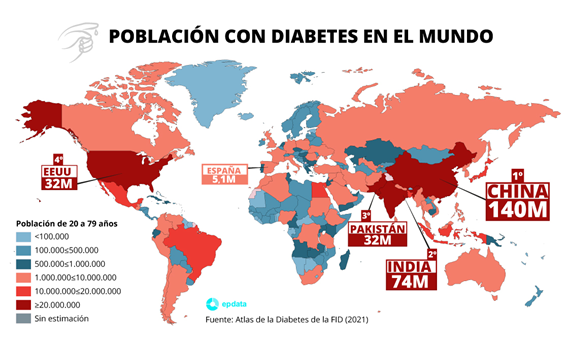
\includegraphics[width=0.8\textwidth]{img/imagen_poblaciondiabetica.png}
    \caption{Población con diabetes en el mundo en 2021 según la FID.}
    \label{fig:poblacion}
\end{figure}



La diabetes puede producirse por dos razones: o no hay suficiente insulina, o bien el cuerpo no responde de forma apropiada a ella. Bajo el primero de los casos, es el páncreas quien no produce la insulina de forma adecuada, por lo que es necesario la aportación de insulina externa para procesar y regular la glucosa en el cuerpo. Si este no responde a ella, lo que nos sitúa en el segundo caso, significa que el hígado no reconoce la insulina que está en el organismo y por tanto, continúa produciendo cantidades inadecuadas de glucosa. Este hecho se conoce como resistencia a la insulina.

\subsection{Tipos de diabetes}
Se describen a continuación los principales tipos de diabetes.

\textbf{Diabetes tipo 1 (DM1)}

Presenta un carácter autoinmune, donde el sistema inmunológico del organismo ataca y destruye las células beta del páncreas, lo que las impide producir insulina, ver Figura \ref{fig:tipos_diabetes}. Por tanto, los pacientes diabéticos de tipo 1 requieren de la administración de insulina externa a través de inyecciones o bombas de insulina. Es la más registrada en niños y adultos jóvenes. Es el caso de este estudio.

\textbf{Diabetes Tipo 2 (DM2)}

Se caracteriza por la resistencia a la insulina y una producción insuficiente de esta, siendo la forma más común de diabetes. Suele ir acompañada de obesidad. A diferencia del caso anterior, las células del cuerpo si que responden a la insulina, pero no lo hacen de forma eficaz, lo que desemboca en niveles elevados de glucosa en sangre (Figura \ref{fig:tipos_diabetes}). La enfermedad parece estar ampliamente relacionada, además de con el sobrepeso,  con otros factores del estilo de vida, como la falta de actividad física o una dieta poco saludable. Por tanto, los pacientes no suelen requerir de inyecciones de insulina, sino que el tratamiento engloba la dieta, el ejercicio y la medicación (donde destacan los antidiabéticos orales). 

\textbf{Diabetes gestacional}

Esta modalidad es un tipo especial de diabetes que se desarrolla durante el embarazo, y se caracteriza por presentar resistencia a la insulina, que parece estar causada por cambios hormonales. A pesar de que la diabetes gestacional suele desaparecer tras el parto, se ha relacionado con un mayor riesgo de que estas mujeres desarrollen diabetes tipo 2 en el futuro. Se puede obtener más información en  \cite{giarllarielli2023diabetes}.

\begin{figure}[h]
    \centering
    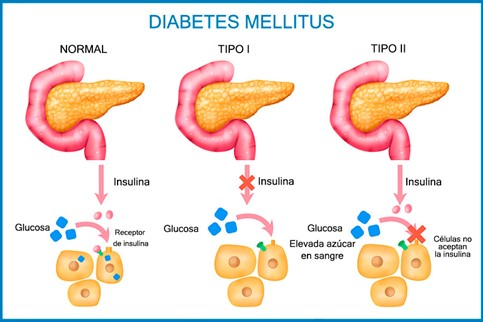
\includegraphics[width=0.6\textwidth]{img/imagen_tipos_diabetes.jpg}
    \caption{Interacción glucosa - insulina sin diabetes y con diabetes.}
    \label{fig:tipos_diabetes}
\end{figure}

\subsection{Rangos diabéticos}

Se incluyen a continuación los rangos que delimitan la diabetes \footnote{Obtenidos de \cite{mayoclinic_prediabetes}}: 

\begin{table}[htbp]
    \centering
    \caption{Valores estipulados para el paciente base.}
    \begin{tabular}{|c|c|c|}
        \hline
          & Ayunas & Tras ingesta  \\
        \hline
        Valores normales & 70-100 mg/dL & <180 mg/dL  \\
        Prediabetes & 100-125 mg/dL & 180-200 mg/dL \\
        Diabetes & >125 mg/dL & >200 mg/dL \\
        \hline
    \end{tabular}
    \label{tab:rangos_diabeticos}
\end{table}

\section{Pruebas glucémicas}

La medición de la glucosa sanguínea constituye el marco para el tratamiento eficaz de hiperglucemias e hipoglucemias en el organismo, así como para el seguimiento de pacientes con patologías relacionadas, incluso, con los avances tecnológicos actuales, para el monitoreo del ejercicio y otras perturbaciones \cite{gygliola2020glucose}. Su clasificación se basa en el método de administración empleado. Así, destacan dos pruebas, la de tolerancia oral a la glucosa y la de tolerancia intravenosa de la glucosa.
La prueba \textbf{Intravenous Glucose Tolerance Test (IGVTT)} es un test médico utilizado para evaluar cómo el cuerpo maneja la glucosa administrada por vía intravenosa. Se emplea principalmente para el diagnóstico de diabetes, aunque también sea útil para identificar otras condiciones relacionadas con la glucosa e insulina. Se administra una cantidad específica de glucosa al organismo mediante una vía, y posteriormente se toman muestras de sangre en intervalos regulares para medir los niveles de glucosa e insulina. Esta prueba permite una evaluación detallada de la función beta-pancreática y de la sensibilidad a la insulina, y, a diferencia de otras pruebas, es más controlada, ya que evita las variaciones en la absorción intestinal de la glucosa.\label{sec:IGVTT} 
La prueba de \textbf{tolerancia oral a la glucosa OGTT} emplea la vía oral para la administración de glucosa. Su principal uso es el diagnóstico de la diabetes tipo 2, pero se usa una variante de esta para identificar diabetes gestacional. Una vez pasado el intervalo de tiempo necesario, se procede de la misma forma que en la anterior prueba, es decir, mediante la extracción de sangre, lo que permite medir los niveles glucémicos. La OGTT identifica modalidades diabéticas clasificando la ingesta del paciente en función de su edad y condición (ver Figura \ref{fig:tipos_OGTT}).  Mientras que en adultos se estima una solución de unos 8 onzas con 75 gramos de azúcar, para niños, la dosis se calcula en función de su peso (1,75 g/kg), con una dosis máxima de 75 gramos. A diferencia de estas dos pruebas, cuya duración suele ser de 2 horas, existe una tercera modalidad empleada para las embarazadas, que utiliza una solución de 8 onzas con 100 gramos de azúcar, y dura 3 horas. \label{sec:OGTT}
\clearpage
\begin{figure}[htbp]
    \centering
    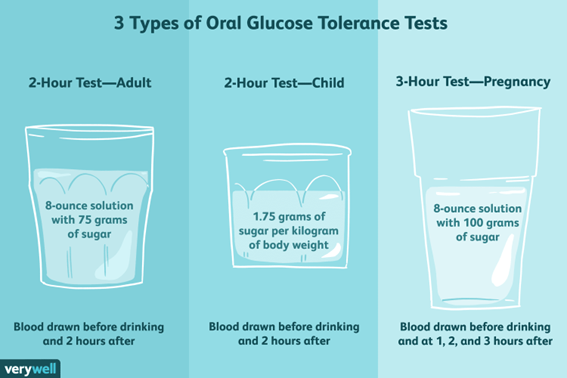
\includegraphics[width=0.75\textwidth]{img/tipos_OGTT.png}
    \caption{Tipos de pruebas de Tolerancia Oral a la Glucosa según el paciente implicado.}
    \label{fig:tipos_OGTT}
\end{figure}

\section{Monitorización y regulación de la glucosa}

\textbf{Sistemas de monitorización }

Se trata de dispositivos que obtienen una lectura de los valores glucémicos del paciente, mediante su monitorización. Se clasifican en tres:
\begin{enumerate}
    \item[-] Monitores de glucosa en sangre (BGM) son los más sencillos y requieren de una gota de sangre del paciente, obtenida mediante una punción del dedo. La sangre se aplica a una tira reactiva insertada en el medidor, que luego muestra la lectura de glucosa. 
    \item[-] Monitores continuos de glucosa (CGM) emplean un sensor insertado bajo la piel, generalmente bajo el brazo, que mide los niveles de glucosa en el líquido intersticial cada pocos minutos. Los datos obtenidos se envían a un dispositivo. A diferencia del monitor anterior, proporciona datos continuos, pero necesitan ser remplazados regularmente. \label{sec:CGM}
    \item[-] Monitores de glucosa flash (Flash Glucose Monitor), similares a los anteriores, a diferencia de que es el propio paciente quien debe escanear el sensor con un lector para poder obtener la lectura. 
\end{enumerate}

Se incluyen en la Figura \ref{fig:sist_mon_2022} los sistemas de monitorización de glucosa  (MCG) comercializados en España en 2022 según \cite{revistadiabetes_monitorizacion_glucosa}:

\begin{figure}[h]
    \centering
    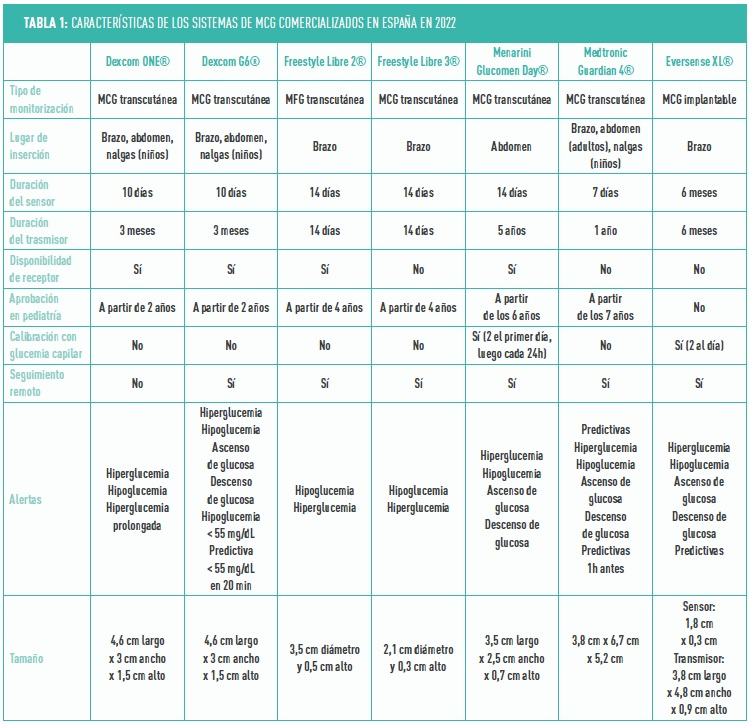
\includegraphics[width=1\textwidth]{img/comercializados.jpg}
    \caption{Sistemas de monitorización de glucosa comercializados en España en 2022.}
    \label{fig:sist_mon_2022}
\end{figure}

\textbf{Bombas de insulina} \label{sec:bomba}

Se trata de dispositivos que administran al organismo insulina, llamada insulina exógena, de manera continua o en dosis, a través de un catéter insertado debajo de la piel. El objetivo de este tratamiento es imitar el funcionamiento del páncreas de una persona sin diabetes. Funcionan de manera similar a un páncreas artificial, proporcionando una infusión constante de insulina basal (programada previamente por el equipo diabetológico, el paciente y/o su familia basándose en los controles de glucemia), así como dosis adicionales o "bolos" de insulina en momentos específicos, como en las comidas, según las necesidades del usuario. Estos bolos también se emplean para corregir las hiperglucemias \footnote{Información obtenida de \cite{FundacionParaLaSalud}.}.
Basándose en los datos de glucosa proporcionados por sistemas de monitorización, como el CGM mencionado anteriormente (Sección \ref{sec:CGM}), se pueden ajustar las configuraciones de esta bomba para adaptarse a necesidades individuales de cada paciente, programando mediante sistemas de control, por ejemplo, diferentes tasas de administración de insulina según la hora del día, la actividad física, etc. 
Entre las principales ventajas de las bombas de insulina, se encuentran cuatro:
\begin{enumerate}
    \item Permite ajustar mejor las diferentes necesidades de insulina que existen en el día gracias a la capacidad para programar las perfusiones basales.
    \item La bomba utiliza análogos de insulina de acción rápida, lo que asegura un efecto más predecible, en comparación con las insulinas de acción lenta o intermedia.
    \item Generalmente, se reduce el riesgo de hipoglucemias graves.
    \item Ha demostrado en diferentes estudios una mejoría en la calidad de vida del niño/adolescente y de su familia. Esta mejora se debe fundamentalmente a la flexibilidad horaria que ofrece.
\end{enumerate}

Sin embargo, también cuenta con algunas desventajas:
\begin{enumerate}
    \item Durante la terapia con bomba el depósito de insulina es muy escaso. Por este motivo se es más susceptible de presentar cetoacidosis en el caso de interrupción en el suministro de insulina.
    \item La bomba se debe llevar las 24 horas del día lo que para algunas personas supone una mayor “atadura” a su diabetes.
    \item Supone mayor gasto que la terapia con múltiples dosis de insulina.
\end{enumerate}


\textbf{Insulina exógena} 

Las insulinas se clasifican atendiendo, principalmente, a la duración de sus efectos así como a la rapidez de su acción, distinguiendo la acción rápida, corta, intermedia, larga o muy larga. Más comúnmente, esta clasificación se reduce a 3 tipos de insulina exógena: acción rápida, media y prolongada. \label{sec:ins_ex}

\begin{enumerate}
    \item[-] \textit{La insulina de acción rápida} produce efecto entre los 5 y 20 minutos desde la administración, ya que se absorbe rápidamente desde el tejido adiposo. Esta cifra resulta un tiempo muy reducido, mientras que su pico de acción se produce aproximadamente a la hora o dos horas del inicio. Su duración en el organismo es de unas 4-6 horas. Se emplea para regular los niveles de glucosa durante las comidas, o bien para corregir niveles altos de esta en sangre.
    Unas pocas unidades pueden durar 4 horas o menos, mientras que 25 o 30 unidades pueden durar 5 a 6 horas. Destacan la insulina lispro, la aspart y la glulisina; y su uso es cada vez más extendido. \label{sec:ins_rap}
    \item[-] \textit{La insulina de acción intermedia} muestra el inicio de acción más tarde, pues se absorbe más lentamente (entre la primera y la segunda hora), así como su pico de acción (a las 4-12 h). Sin embargo, su duración es sustancialmente mayor, alcanzando las 12-18 horas. Se usa para controlar el azúcar por la noche o bien entre las comidas. Destaca la insulina NPH.
    \item[-] \textit{La insulina de acción prolongada} se administra a pacientes diabéticos tipo 1 cuyo valor de insulina ha de mantenerse constante para todo el día. El inicio de la acción se produce tras 1 hora de la ingesta aproximadamente y, a diferencia del resto de insulinas, no experimenta picos de acción, sino que muestra un comportamiento estable. En general, se usa para controlar el azúcar a nivel diario. Ejemplos de esta insulina son Glargina y Detemir. \label{sec:ins_prol}
\end{enumerate}

\textbf{Páncreas artificial} 
\label{sec:pancreas_artificial}

Un páncreas artificial es un sistema en lazo cerrado automatizado para la administración de insulina en el organismo que imita la manera en que un páncreas sano controla la glucosa en la sangre.
Este sistema está formado por tres componentes (ver Figura \ref{fig:pancreas_art} \footnote{Obtenido de \cite{vibora2017pancreas}}):
\begin{enumerate}
    \item[-] Un monitor continuo de glucosa o CGM anteriormente expuesto en la Sección \ref{sec:CGM}, que  lleva un registro de la concentración de glucosa en la sangre cada pocos minutos mediante un pequeño sensor que se inserta debajo de la piel. El sensor envía la información de forma inalámbrica a un programa almacenado en un teléfono inteligente o en una bomba de infusión de insulina. Este dispositivo garantiza la continua monitorización de las concentraciones de glucosa.
    \item[-] Un programa informático, que calcula cuánta insulina se necesita y envía una señal a la bomba de infusión de insulina cuando debe administrarse. Así, el programa mejora el control de la glucosa en la sangre ajustando automáticamente la cantidad de insulina que administra para mantener las concentraciones de glucosa en la sangre dentro del rango. El modelado del comportamiento de la glucosa en el organismo mediante relaciones matemáticas, como las que se analizan en esta memoria, permiten diseñar sistemas de control adecuados y eficientes que será los que se implementen como parte del programa informático. Precisamente, el estudio de los modelos matemáticos y los sistemas de control más sencillos son el objetivo de este trabajo.
    \item[-]  La bomba de infusión de insulina, que administrará pequeñas dosis de insulina a lo largo del día cuando las concentraciones de glucosa en sangre no estén dentro de su rango objetivo (Sección \ref{sec:bomba}).
\end{enumerate}

\begin{figure}
    \centering
    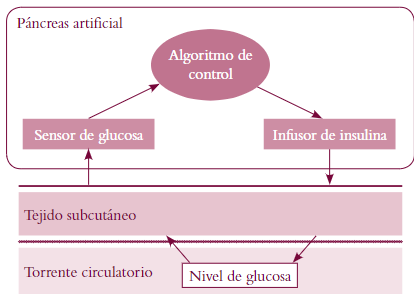
\includegraphics[width=0.65\linewidth]{img/pancre.PNG}
    \caption{Sistema de control del páncreas artificial.}
    \label{fig:pancreas_art}
\end{figure}

Existen diferentes tipos de sistemas de páncreas artificial, entre ellos: 
\begin{enumerate}
    \item[-] \textit{Sistemas de umbral de suspensión y de suspensión predictiva}, que pueden suspender de forma temporal la administración de insulina si la concentración de glucosa en sangre es muy baja, y evitar así una posible hipoglucemia.
    \item[-] \textit{Sistemas de insulina}, de carácter híbrido, que ajustan automáticamente las dosis de insulina en función de los valores leídos gracias al sistema de monitorización. Para estos sistemas, es necesario que el paciente cuente las concentraciones de ingesta y calcule la dosis necesaria para las comidas.
    \item[-] \textit{Sistemas hormonales duales}, en desarrollo, que emplean la insulina y el glucagón para reducir y aumentar las concentraciones de glucosa en sangre, respectivamente. Este comportamiento simula el del páncreas, y se estiman buenos resultados para ellos. 
\end{enumerate}

Mediante el empleo de modelos matemáticos que explican la interacción glucosa – insulina, se pretende en este análisis estudiar el comportamiento de la glucosa en el organismo, así como emplear estrategias de control para regular los niveles basales glucémicos.

\section{Modelos matemáticos del sistema glucorregulatorio}

\subsection{El Modelo de Ackerman}

\subsubsection{Contexto, funcionamiento y finalidad del modelo}

Constituye el primer intento de modelización de los procesos fisiológicos durante la metabolización de la glucosa, y se llevó a cabo en los años 60. Se trata de un modelo lineal cuya finalidad era la detección de la diabetes.
El Modelo de Ackerman se basa en la prueba OGTT de tolerancia oral a la glucosa (explicada en la Sección \ref{sec:OGTT}), cuyas mediciones servirán para obtener el diagnóstico de la enfermedad. El objetivo además era construir un modelo que describiese con precision el sistema regulador de la glucosa en la sangre durante la prueba OGTT. Además del empleo de esta prueba, se debe medir el péptido C para calcular la secreción de insulina, ya sea por desconvolución o modelado matemático.
Este modelo emplea la información proporcionada por dos concentraciones sanguíneas: la concentración de la glucosa y la de la insulina, englobando esta ultima un conjunto de hormonas. En \cite{ackerman1965model}, Ackerman interpretará que las hormonas que hacen disminuir la concentración de glucosa incrementarán la insulina, mientras que las que hacen el efecto contrario (elevar la glucosa), disminuirán los niveles de insulina. Por tanto, su conocimiento sobre la fisiología de la insulina y la glucosa en nuestro organismo fue clave para desarrollar el modelo. Aun así, como todos los modelos, presenta inconvenientes, principalmente en relación con el tiempo transcurrido respecto a la ingesta de glucosa.

\subsubsection{Ecuaciones y parámetros del Modelo de Ackerman}

El modelo es muy simple ya que requiere un número limitado de muestras de sangre durante la prueba OGTT. Da origen a un sistema de ecuaciones diferenciales prestando atención a dos concentraciones:

\begin{enumerate}
    \item[-] la concentración sanguínea de glucosa G(t), y
    \item[-] la concentración de insulina en plasma I(t).
\end{enumerate}

Las dos ecuaciones del modelo son:

\begin{equation}
\frac{dG(t)}{dt} = -p_1 (G(t)-Gb)-p_2 (I(t)-Ib)
\end{equation}

\begin{equation}
\frac{dI(t)}{dt} = p_4 (Gb-G(t))-p_3(I(t)-Ib) 
\end{equation}

En ellas, $p_1$, $p_2$, $p_3$ y $p_4$ son parámetros del modelo, mientras que $G_b$ e $I_b$ son los niveles de glucosa e insulina basal, respectivamente. 

	

\subsection{El Modelo Mínimo de Bergman}
\subsubsection{Contexto, funcionamiento y finalidad del modelo}
Este modelo aparece en 1980 de la mano de Richard N. Bergman y su equipo, y representa el verdadero inicio del modelado de las dinámicas glucosa - insulina. 
Su aparición se debe al aumento de los trastornos de sensibilidad de los tejidos a la insulina en diversas condiciones patológicas, como la diabetes (aunque también la obesidad o las enfermedades cardiovasculares), lo que hizo necesario trabajar en la cuantificación, mediante un proceso no invasivo, de la sensibilidad a la insulina. Se desarrolló entonces una prueba denominada con las siglas IVGTT (Sección \ref{sec:IGVTT}) para medir esta sensibilidad, basada en la administración intravenosa de un bolo de glucosa y el muestreo frecuente de las concentraciones tanto de glucosa como de insulina en el paciente. La interpretación de esta prueba se lleva a cabo mediante el modelo fisiológico que titula este apartado: el Modelo Mínimo.

Este modelo interpreta el organismo como un único compartimento, que posee una concentración basal tanto de glucosa como de insulina. Se basa en dos partes: 
\begin{enumerate}
    \item Estudia la cinética de la glucosa; es decir, describe la evolución (en tiempo) de la concentración plasmática de glucosa. Responde a la pregunta de cómo reacciona la concentración de glucosa a la acción de la insulina.
    \item Analiza la cinética de la insulina; lo que implica la medición de la concentración de insulina en el plasma en función del tiempo. Esto se traduce en la dinámica de liberación de insulina pancreática en respuesta al estimulo de un aporte de glucosa. Responde a la pregunta de cómo reacciona la insulina a la concentración de la glucosa en sangre. Introduce además el efecto de una nueva variable: la insulina activa, X(t).  De naturaleza “artificial”, se encuentra relacionada con dicha concentración insulínica pero que no coincide exactamente con ella.
\end{enumerate}

El análisis del comportamiento del sistema glucorregulatorio ha sido llevado a cabo mediante este modelo, y el procedimiento se encuentra en las siguientes secciones.

\section{La ingeniería de control}

La ingeniería de control se define por Jose García - Tirado en \cite{tirado2016ingenieria} como la disciplina que hace uso de la teoría de control para diseñar sistemas que garanticen el comportamiento deseado de otros. La \textit{teoría de control} estudia, por tanto, el comportamiento de estos sistemas dinámicos y la manera de lograr que se comporten como se desea. El término \textit{sistema} en este contexto se refiere a un mundo donde se producen tanto entradas (perturbaciones, exitaciones) como salidas (que se denominan respuestas).

\subsection{Principios básicos de la ingeniería de control}

La ingeniería de control se basa en ciertos principios básicos. 

La \textit{\textbf{estabilidad del sistema}}, en primer lugar, consiste en la capacidad del sistema para mantener el comportamiento deseado a lo largo del tiempo, en respuesta a perturbaciones o bien a cambios en las condiciones iniciales. Un sistema estable volverá a su estado de equilibrio tras la perturbación. En este contexto, un sistema con capacidad inherente de ajustarse y mantener su salida dentro de unos límites, sin necesidad de intervención externa se denomina \textbf{\textit{proceso autorregulador}}. Básicamente, un proceso autorregulado es aquel que tiende a estabilizarse pot si mismo. Es el caso del control de los niveles de la glucosa en el organismo.

La \textit{\textbf{retroalimentación}} es un mecanismo de control que permite a los sistemas ajustar su comportamiento. Mediante su uso, la información de entrada (\textit{variable de entrada}) se contrasta con un \textit{valor referencia} (llamado consigna de control) para darle una orden a la \textit{variable manipulada} y ejecutar así una acción correctiva. Se pueden dar dos tipos de retroalimentación:
\begin{enumerate}
    \item[-] Si la retroalimentación es \textit{negativa}, se reduce la diferencia entre la salida deseada y la salida real del sistema, estabilizando el sistema, y mejorando su precisión y resistencia a perturbaciones.
    \item[-] Si la retroalimentación es \textit{positiva}, al aumentar la diferencia entre la salida deseada y la real, se obtienen sistemas más inestables, generando respuestas oscilatorias, entre otras. 
\end{enumerate}

\subsection{Control de la glucosa en el organismo}

El el contexto biomédico, el conocimiento del funcionamiento de diferentes mecanismos fisiológicos del cuerpo humano en respuesta a perturbaciones ha experimentado una mejora significativa. Se entiende un \textit{ser vivo} como un conjunto de controladores automáticos internos que hacen su trabajo de manera colaborativa y distribuida, concepto comprensible, por ejemplo, con mecanismos básicos como la regulación del pH o de la temperatura, donde es el propio organismo quien regula estas variables y las mantiene en límites adecuados. Gracias al modelado matemático, se ha logrado una mejora en la comprensión de complejidad de los sistemas biológicos, destacando las metodologías automatizadas, que diseñan e implementan sistemas de control de manera automática, reduciendo la intervención manual y mejorando tanto la eficiencia como el desarrollo del sistema. Pese a que existen diferentes rutas para 'cerrar el lazo', J. Bondia estima en \cite{bondia2010pancreas} que la más adecuada es la que comprende la monitorización continua de glucosa subcutánea (s.c -s.c) visible en la Figura \ref{fig:ruta_sc}, destacando respecto a otras rutas como la intravenosa o la intraperitoneal.
\clearpage
\begin{figure}[htbp]
    \centering
    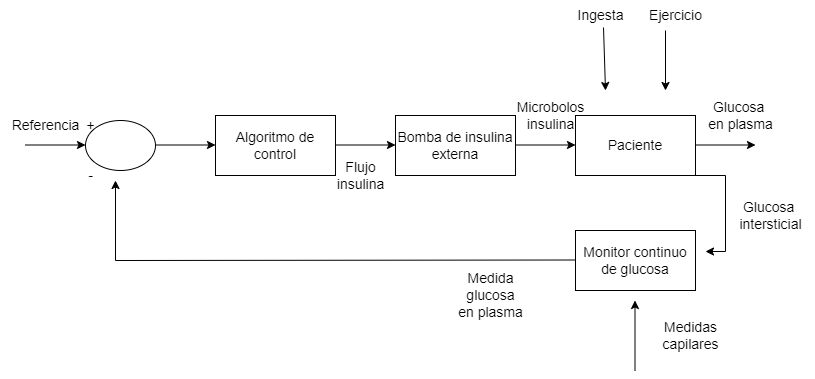
\includegraphics[width=1\linewidth]{img/ruta_sc.png}
    \caption{Lazo de control básico en la ruta s.c. -s.c. Fuente propia.}
    \label{fig:ruta_sc}
\end{figure}

J. Bondía también habla del problema de la sobreactuación, que es especialmente significativo en la compensación de ingestas, donde los errores son grandes. Es por ello, indica, que se emplea con frecuencia el anunciamiento de comidas, donde el paciente indica el instante y la cantidad de ingesta, como se hace en este trabajo. Pese a que, como se ha comentado, la ingesta no es una perturbación medible del todo, pues el flujo de absorción intestinal de glucosa solo se puede estimar en condiciones experimentales, la única información de la que se puede disponer es el instante de inicio de la ingesta y la estimación de la cantidad de hidratos de carbono por parte del paciente. Se muestra en la Figura \ref{fig:ruta_mod} el lazo de control modificado para esta condición, denominada, en la teoría de control, feedforward. Esta se combina siempre con una estrategia de realimentación como la vista antes (o feedback).
\clearpage
\begin{figure}[htbp]
    \centering
    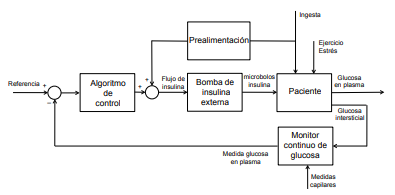
\includegraphics[width=1\linewidth]{img/ruta_mod.png}
    \caption{Lazo de control con anunciamiento de comida. Fuente propia.}
    \label{fig:ruta_mod}
\end{figure}

En el contexto de la glucosa, dispositivos como el páncreas artificial basan su funcionamiento en la ruptura del lazo de control natural. Este concepto se refiere a la estructura mediante la cual se regula el comportamiento de un sistema, mediante componentes que mantienen las variables dentro de rangos deseados. El estado natural de los sistemas de regulación del cuerpo humano es el lazo cerrado donde la acción de control se ajusta continuamente en función de la retroalimentación de la salida del sistema. La salida se mide y se compara con el valor deseado, y cualquier desviación (error) se utiliza para corregir la acción de control, mejorando la precisión y la estabilidad del sistema. Cuando se altera el comportamiento del organismo, como es el caso de la falta de insulina, que se traduce en hiperglucemia, se pasa al lazo de control abierto, donde la acción de control se aplica directamente sin usar retroalimentación para corregir el error entre la salida real y la deseada. Esto resulta en un estado de vulnerabilidad permanente hacia condiciones de alta o de baja concentración de glucosa.

Por tanto, la aplicación de principios de control automático en la diabetes representa un avance significativo y necesario en el área de la medicina, permitiendo un manejo más efectivo y preciso de la enfermedad, mejorando la calidad de vida de los pacientes y reduciendo el riesgo de complicaciones a largo plazo.

\clearpage
\section{Estado del arte y trabajos relacionados}

Respecto a las relaciones matemáticas de los mecanismos biológicos de la glucosa e insulina, la realidad es que actualmente existen multitud de modelos que simulan cada vez de forma más precisa su comportamiento. Además de los modelos clásicos, entre los que destacan los mencionados Modelos de Bergman y Ackerman, han surgido gran variedad de ellos.
\begin{enumerate}
    \item A nivel matemático, modelos basados en redes neuronales y Machine Learning, mediante la aplicación de nuevas inteligencias artificiales que son capaces de predecir los niveles de glucosa. Se incluyen entre ellos modelos basado en redes neruonales convolucionales CNN, que identifican patrones y mejoran las predicciones de los niveles de glucosa (\cite{carrillo2021long}), o 
    modelos de redes neuronales a corto plazo, como el 
    MLP (Multi Layer Perceptron), que es un tipo de red neuronal artificial que realiza predicciones a corto plazo de niveles de glucosa futuros permitiendo el mejor ajuste del tratamiento insulínico. Sus resultados son positivos, más información en \cite{allam2011recurrent}.
    \item En el ámbito probabilístico, modelos estocásticos que preveen las variaciones de la glucosa, entre los que se encuentran los modelos de Markov, procesos Gaussianos y modelos ARIMA. Se obtienen las probabilidades de que un paciente supere ciertos umbrales críticos en \cite{caperamodelo}, estimando relaciones relevantes entre los datos.
    \item En el ámbito médico, se han realizado grandes cohortes (estudios longitudinales), como el llevado a cabo por Leticia Marques da Silva Neto y otros \cite{da2024asociacion} en relación a la glucemia inestable y la mortalidad.
    \item En el ámbito farmacéutico, destacan las terapias combinadas de insulina con otros medicamentos \footnote{Más información en \cite{karam2024capitulo}}.
    \item A nivel tecnológico, se avanza en sistemas de monitoreo continuo de glucosa, así como, por excelencia, en el páncreas artificial. Destaca la empresa de tecnología médica Dexcom, cuyo mayor activo son los dispositivos Dexcom G6 y G7 de control de glucosa que permiten un monitoreo constante y a tiempo real. Su integración en aplicaciones móviles, así como la configuración de múltiples ventajas como alarmas y alertas personalizadas a los niveles glucémicos de cada paciente consolidan este producto como uno de los más potentes del mercado. Dexcom G7 se ha consolidado como el sistema MCG más rápido del mercado, pues requiere unicamente de 30 minutos para calentase, además de haber reducido un 60\% su tamaño respecto del anterior. Muy recientemente se ha aprobado la comercialización de un sistema Dexcom para diabéticos tipo 2 \cite{infobae_monitor_glucosa}, que es de venta libre, a diferencia del resto, que son bajo receta. Los sensores FreeStyle también permiten llevar un control continuo de los niveles de glucosa, y recientemente se ha estimado que los diabéticos tipo 2 con esta tecnología combinada con tratamientos con antagonistas del GLP 1 obtienen mejores resultados que solo con estos antagonistas (\cite{immedicohospitalario_freestyle}).
\end{enumerate}

Respecto al páncreas artificial, en el mes de abril se aprobó un nuevo páncreas para diabéticos tipo 1 que reduce los esfuerzos del paciente. Se trata de un sistema híbrido en lazo cerrado que adecua por si mismo los niveles de glucosa en el organismo, alejando al paciente de la preocupación ante esta posible situación. Este sistema emplea un sensor subcutáneo para monitorear los niveles de azúcar en sangre y una bomba de insulina inalámbrica para su administración \footnote{Para más información, consultar en \cite{gizmodo_pancreas_artificial}.}.

\capitulo{4}{Metodología}

Los modelos y simulaciones analizados a continuación simplifican el funcionamiento del sistema glucorregulatorio de nuestro organismo. Su finalidad es estudiar el comportamiento y efecto de dicho sistema, quedando fuera de este estudio, la definición de nuevos criterios para establecer rangos o parámetros específicos de la interacción entre la glucosa y la insulina. De esta forma, el modelado de la glucosa permite observar cómo afectan ciertas variables a su comportamiento.

\section{Descripción de los datos}
Se presenta un estudio que modela el comportamiento de la glucosa e insulina para pacientes no diabéticos y diabéticos. Se han seleccionado para ello, dos pares de valores de glucosa e insulina basal, uno para cada tipo de paciente. Esta elección ha sido realizada teniendo en cuenta los rangos diabéticos mostrados en la Tabla  \ref{tab:rangos_diabeticos}, así como teniendo en cuenta lo mencionado por Jaime Carrillo Moreno y otros en \cite{carrillo2021long}. De esta manera, se considera que representan adecuadamente las características propias de su grupo.

La glucosa se mide en mg /dL. La inclusión de esta variable en el modelo se realiza en mmol/L, lo que implica el uso de factores de conversión. La relación entre ambas unidades se basa en que 1 mmol/L = 18 mg/dL.
La insulina se mide en mU /L.
Los parámetros de los modelos empleados en el análisis han sido seleccionados en base a su uso en estudios previos, garantizando su validez debido a que han demostrado ser efectivos y relevantes en investigaciones anteriores sobre diabetes y sus marcadores.

Se presentan en la siguientes tablas, Tabla \ref{tab:valores_no_diabetico} y Tabla \ref{tab:valores_diabetico}, los valores estimados para el paciente no diabético y para el paciente diabético.

\begin{table}[htbp]
    \centering
    \caption{Valores basales estimados para el paciente base.}
    \begin{tabular}{|c|c|c|}
        \hline
          & Valor\\
        \hline
        Gb & 81 mg/dL \\
        Ib & 12 mU/L  \\
        \hline
    \end{tabular}
    \label{tab:valores_no_diabetico}
\end{table}
\begin{table}[htbp]
    \centering
    \caption{Valores basales estimados para el paciente diabético.}
    \begin{tabular}{|c|c|c|}
        \hline
          & Valor\\
        \hline
        Gb & 126 mg/dL \\
        Ib & 10 mU/L  \\
        \hline
    \end{tabular}
    \label{tab:valores_diabetico}
\end{table}

\subsection{Parámetros glucémicos empleados en el análisis}

Los valores asignados a los parámetros incluidos en los modelos para este estudio son los establecidos por \cite{fisher1991semiclosed}.

\begin{table}[htbp]
    \centering
    \caption{Valores de los paráemtros glucémicos de los modelos de la glucosa.}
    \begin{tabular}{|c|c|c|}
        \hline
        Parámetro & Valor& Unidad \\
        \hline
        $p_1$ & 0.028 & $min^{-1}$ \\
        $p_2$ & 0.025 & $min^{-1}$ \\
        $p_3$ & 0.000013 &  $min^{-2} (\mu UI / mL)$\\
        $p_6$ & 0.003349 & $min^{-1}$ \\
        n & 5/54 & $min^{-1}$ \\
        $V_i$ & 12 & L \\
        \hline
    \end{tabular}
    \label{tab:parametros_glucemicos}
\end{table}

\section{Modelo de Bergman}

Este modelo refleja el comportamiento del sistema glucorregulatorio de un \textbf{paciente sano}. El Modelo Mínimo se basa en la regla de balance de masa, que indica que la cantidad acumulada en un compartimento es exactamente:
\begin{equation}
acumulado = \text{cantidad entrada - cantidad salida + generado - consumido}
\label{eq:balance_masas}
\end{equation}
 Está formado por 2 ecuaciones diferenciales no lineales definidas por Bergman en \cite{bergman1979quantitative}, que estudian el comportamiento de la Glucosa G(t) y de la Insulina Activa X(t) a lo largo del tiempo \footnote{Información referente a este modelo ha sido comprendida gracias al desarrollo propuesto en \cite{perez2017analisis}}.
 Como se ha comentado antes, se remarca la importancia de la diferencia entre estas dos variables. Mientras que \textit{insulina activa} es la parte de insulina lista para ser utilizada por el cuerpo para regular los niveles de azúcar en sangre, la \textit{insulina normal} es la forma 'inactiva' o almacenada en la hormona. Cuando es necesario, el organismo convierte la insulina normal en activa para cumplir sus funciones. 
\begin{align}
    \frac{dG(t)}{dt}= -p_1 (G(t) - G_b) - X(t)G(t) , G(0) = Gb
    \label{eq:ecBergGluc}\\
    \frac{dX(t)}{dt}= -p_2 X(t) + p_3(I(t) - I_b),    X(0) = 0
    \label{eq:ecBergInsAc}
\end{align}

De esta manera, para la ecuación de la insulina activa X(t), el primer témino representa la velocidad a la que esta se elimina en el cuerpo, mientras que la segunda parte de la ecuación representa la velocidad de transformación de insulina a insulina activa. La diferencia presente en esta parte de la ecuación refleja esta conversión. Si la concentración de insulina en un momento dado es mayor que la basal (I(t)>$I_b$), la diferencia será positiva, lo que supone un estímulo para la conversión a insulina activa. Por otro lado, si la insulina total es menor que la basal (I(t) <$I_b$), la diferencia será negativa, lo que supone un estímulo para la liberación de insulina en sangre, en vez de la conversión a insulina activa. 

El resto de variables y parámetros del modelo se definen a continuación:
\begin{enumerate}
    \item[-] $G_b$: valor de glucosa basal (cte.).
    \item[-] $I_b$: valor de insulina basal (cte.).
    \item[-] $p_1$: valor máximo inicial de la curva de interacción glucosa- insulina (cte.).
    \item[-] $p_2$: tasa disminución de glucosa en tejido por unidad de insulina (cte.).
    \item[-] $p_3$: tasa de incremento de glucosa después de la acción de la insulina (cte.). 
    \item[-] G(t): concentración de la glucosa en plasma.
    \item[-] I(t): concentración de la insulina en plasma.
    \item[-] X(t): concentración de la insulina activa en plasma.
\end{enumerate}

\subsection{Estabilidad del sistema}
\label{sec:est_estac}

Inicialmente se va a estudiar el comportamiento del modelo bajo condiciones estables, es decir, el sistema en equilibrio. Encontrar las concentraciones de glucosa e insulina en condiciones estables (sin cambios en entradas o en otras condiciones) es un punto clave para el análisis y la compresión de la regulación de la glucosa en el cuerpo humano. Este equilibrio se consigue hallando el estado estacionario del sistema estableciendo las derivadas de las variables a 0. En otras palabras, mediante este método se obtienen los puntos en los cuales las variables del sistema no cambian con el tiempo.
Partiendo de las ecuaciones iniciales, es posible hallar, por tanto, qué valores adoptan las variables G(t) y X(t) en equilibrio dados unos valores iniciales de Glucosa Basal (Gb) e Insulina Basal (Ib), y analizar así el comportamiento del sistema en condiciones estables.
Garantizando su invariabilidad con el tiempo, igualando a 0 \eqref{eq:ecBergGluc} y \eqref{eq:ecBergInsAc} :
\begin{align}
    0= -p_1 (G(t) - G_b) - X(t)G(t) \\
    0= -p_2 X(t) + p_3(I(t) - I_b) 
\end{align}
Para el caso base la condición es que X(0)=0. 
Por tanto, para la insulina activa:
\begin{align*}
    0= -p_2 X(0) + p_3(I(0) - I_b) \\
    0= -p_2 (0) + p_3(I(0) - I_b) \\
    0= p_3(I(0) - I_b) \\
    p_3 I_b= p_3 I(0) \\
    I_b = I(0) \\
\end{align*}

Por otro lado, para la glucosa:
\begin{align*}
    0= -p_1 (G(0) - G_b) - X(0)G(0) \\
    0= -p_1 (G(0) - G_b) - (0)G(0) \\
    0= -p_1 (G(0) - G_b) - 0 \\
    0= -p_1 (G(0) - G_b) \\
    p_1 G(0)= p_1 G_b \\
    G(0) = G_b \\
\end{align*}
Este comportamiento se refleja en la glucosa e insulina activa en la Figura \ref{fig:bergman_en_ayunas}.

\begin{figure}[htbp]
    \centering
    \begin{subfigure}[b]{0.9\linewidth} % Ancho ajustado al 90% del ancho de la línea
        \centering
        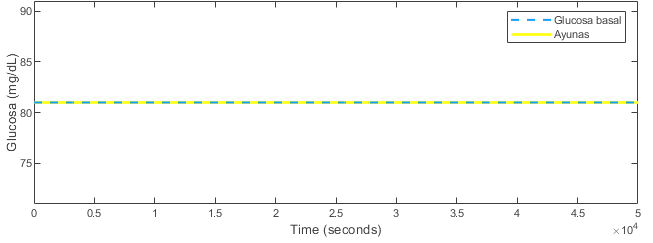
\includegraphics[width=\linewidth]{img/modelo_original/ayuno.png}
        \caption{Glucosa en ayuno.}
        \label{fig:bergman_ayunas_glucosa}
    \end{subfigure}
    
    \vspace{0.5cm} % Espacio vertical entre las subfiguras

    \begin{subfigure}[b]{0.9\linewidth} % Ancho ajustado al 90% del ancho de la línea
        \centering
        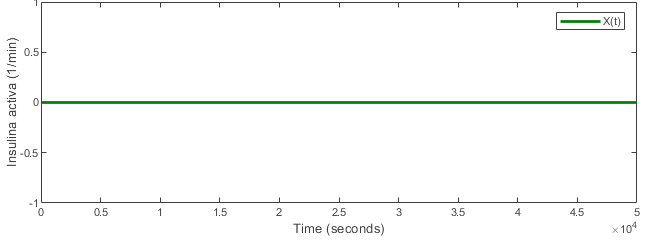
\includegraphics[width=\linewidth]{img/modelo_original/ins_act_ayuno.png}
        \caption{Insulina activa en ayuno.}
        \label{fig:bergman_ayunas_insulina_activa}
    \end{subfigure}
    
    \caption{Comportamiento de la glucosa e insulina activa para una situación en equilibrio, sin perturbaciones. Fuente propia.}
    \label{fig:bergman_en_ayunas}
\end{figure}


De esta forma se define el comportamiento de la glucosa en el organismo para condiciones estables o equilibrio.
Mientras no se reciba ninguna perturbación, la insulina no varía con respecto a la insulina basal, así como la glucosa no varía respecto de la glucosa basal. La insulina activa, por su parte, se ve obligada a mantenerse en 0, pues la insulina I(t) no experimenta ninguna variación.

\subsection{Modelado dinámico de la insulina}

Para el Modelo de Bergman, la insulina no se encuentra modelada, pues se trataba como un vector de medidas a lo largo del tiempo obtenidas tras una ingesta, ya que el modelo estaba pensado para para la prueba IVGTT.

En esta sección, se modifica el tratamiento de la insulina I(t) dentro del modelo, evolucionando de una constante fija a una ecuación que varía con el tiempo. Esta actualización tiene como objetivo emular de manera más precisa el comportamiento dinámico del páncreas en la regulación de los niveles de insulina. Esta implementación de una función variable con el tiempo, obtenida de \cite{alonso2014modelos}, tiene como finalidad reflejar mejor la fisiología del páncreas y su respuesta a los niveles de glucosa.
\begin{equation}
    \frac{dI(t)}{dt} = p_6 (G(t)-p_5)^+ t -n(I(t)+Ib), Ib(0)=0
    \label{eq:insulina_variable}
\end{equation}
La ecuación \eqref{eq:insulina_variable}, que se une al sistema formado por \eqref{eq:ecBergGluc} y \eqref{eq:ecBergInsAc}  modela el comportamiento del páncreas en relación con la liberación de insulina en respuesta a los niveles de glucosa en la sangre, concretamente el término:
\begin{equation}
    Páncreas (t)= (G(t)-p_5)^+ t 
    \label{eq:pancreas}
\end{equation}
Este término se conoce como la “parte positiva” de la diferencia G(t) - $p_5$, donde $p_6$ es la constante de proporcionalidad en la tasa de cambio en la insulina. Mientras que $p_6$ y n se encuentran definidos en la Tabla \ref{tab:parametros_glucemicos}, el parámetro $p_5$ es un valor específico que define el punto en el cual el nivel de glucosa en la sangre se considera lo suficientemente alto como para activar la liberación de insulina por parte del páncreas. Este umbral es un límite crítico que determina si los niveles de glucosa en la sangre están por encima o por debajo del rango normal.
El umbral divide los niveles de glucosa en la sangre en dos regiones distintas: por encima y por debajo de $p_5$.
\begin{enumerate} \label{sec:p5}
    \item[-] Si G(t) > $p_5$, el término \eqref{eq:pancreas}  tiene el valor de G(t) - $p_5$. Esto indica que el nivel de glucosa actual es superior del umbral de glucosa establecido, y por tanto, se debe liberar insulina para reducir los niveles de glucosa. Cuando G(t) = $p_5$, finalizará la liberación.
    \item[-] Si G(t) <= $p_5$, el término \eqref{eq:pancreas} tiene el valor de 0, pues la glucosa no es suficientemente alta como para que sea necesario liberar insulina para reducirla.
\end{enumerate}

Para las siguientes gráficas de Figura \ref{fig:bergman_p5_base}, se observa el comportamiento de la glucosa bajo la liberación de la insulina por parte del páncreas. La raya vertical delimita el umbral de $p_5$. Para este caso, se comienza con una glucosa de 144 mg/gL y un $p_5$ = 117 mg/dL, por lo que G(t) > $p_5$. Cuando $p_5$ se iguala a G(t), el páncreas deja de liberar insulina y su gráfica experimenta una caida hasta volver al nivel basal.
\clearpage
\begin{figure}[htbp]
    \centering
    \begin{subfigure}[b]{0.9\linewidth} % Ancho ajustado al 90% del ancho de la línea
        \centering
        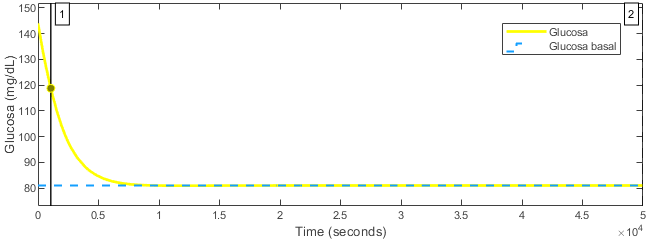
\includegraphics[width=\linewidth]{img/modelo_original/p5_base_gluc.PNG}
        \caption{Glucosa con umbral p5.}
        \label{fig:bergman_p5_glucosa}
    \end{subfigure}
    
    \vspace{0.5cm} % Espacio vertical entre las subfiguras

    \begin{subfigure}[b]{0.9\linewidth} % Ancho ajustado al 90% del ancho de la línea
        \centering
        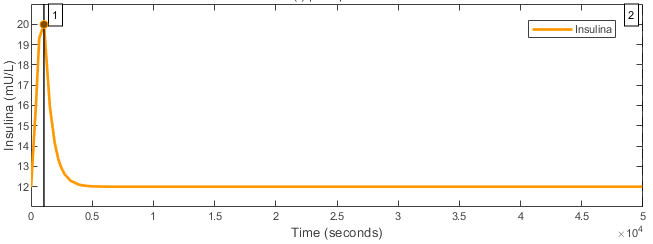
\includegraphics[width=\linewidth]{img/modelo_original/p5_base_ins.PNG}
        \caption{Insulina con umbral p5.}
        \label{fig:bergman_p5_insulina}
    \end{subfigure}
    
    \caption{Efecto de la selección de un umbral p5 determinado para la liberación de insulina. Fuente propia.}
    \label{fig:bergman_p5_base}
\end{figure}



\subsection{Descripción de los parámetros}

El Modelo de Bergman cuenta con 3 parámetros clave para la representación del funcionamiento del sistema glucorregulatorio del organismo: $p_1$, $p_2$ y $p_3$.
\begin{enumerate}
    \item $p_1$ es la tasa de eliminación de la glucosa, y sus valores para un paciente normal oscilan en el rango entre 0.02 – 0.05 $min^{-1}$. 
    
    Un paciente diabético verá disminuido su valor de $p_1$, encontrándose en el límite inferior del rango, incluso quedando por debajo de él.
    
    \item $p_2$ es la tasa de insulina activa, y su rango es el mismo que en el anterior caso (0.02 - 0.05 $min^{-1}$). 
   
    En ayuno, $p_2$  tiende a acercarse al extremo inferior del rango, mientras que, tras la ingesta, el valor aumenta. Para pacientes diabéticos, debido a la disminución de la producción de insulina, así como la disminución de sensibilidad de los tejidos a la insulina, $p_2$  disminuye notablemente.
    
    \item $p_3$ constituye el coeficiente de transformación de insulina a insulina activa, y sus valores oscilan entre $10^{-5}$ y $10^{-6}
    L/mU$ $min ^2$. 
    
    Para pacientes diabéticos, concretamente para DM2, debido a la resistencia a la insulina, el cuerpo produce más insulina, lo que se traduce en un aumento de $p_3$.
\end{enumerate}

De la misma forma, se ha considerado realizar un análisis propio e independiente de estos parámetros, mediante el estudio de su variación, para comprobar que los rangos son correctos, así como que los valores asignados a cada parámetro son adecuados. Los valores modificados se encuentran en el anexo.

\section{Modelo de Bergman Modificado}
\label{sec:indicar_n}
El modelo matemático estudiado en la sección anterior pierde su eficacia cuando el sistema glucosa - insulina ve alterado su comportamiento. En particular, en pacientes diabéticos tipo 1, cuando el páncreas no puede generar insulina, la ecuacion (\ref{eq:pancreas}) no es adecuada. 
Se introduce un modelo modificado,  obtenido en \cite{zamarron2021modelos}, que incluye la insulina exógena U. Este nuevo comportamiento se representa mediante una nueva ecuación para el Modelo de Bergman, que adopta una nueva implementación para I(t).
\begin{align}
    \frac{dG(t)}{dt}= -p_1 (G(t) - G_b) - X(t)G(t), G(0)=Gb \\ \label{eq:glucosa_mod_mod}
    \frac{dX(t)}{dt}= -p_2 X(t) + p_3(I(t) - I_b), X(0) = 0 \\
    \frac{dI(t)}{dt}= -n I(t) + \frac{U(t)}{Vi}, I(0) = Ib 
    \label{eq:ecBergMod}
\end{align}
Donde:
\begin{enumerate}
    \item[-] \textbf{1/n} es la constante de tiempo del sistema, e indica el tiempo que tarda la insulina en alcanzar el valor de la insulina exógena administrada (cte.). 
    \item[-] \textbf{Vi} es el volumen de distribución de insulina (cte.). 
    \item[-] \textbf{U(t)} es insulina exógena que se administra. 
\end{enumerate}

En la Figura \ref{fig:modificado_comportamiento_ayuno} se muestra el comportamiento de la glucosa e insulina para un paciente diabético tipo 1 en ayunas que no recibe administración de insulina exógena.

\begin{figure}[htbp]
    \centering
    \begin{subfigure}[b]{0.9\linewidth} % Ancho ajustado al 90% del ancho de la línea
        \centering
        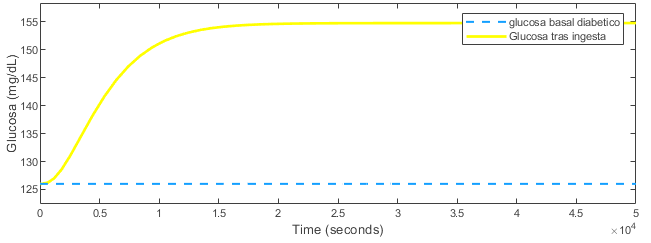
\includegraphics[width=\linewidth]{img/modelo_modificado/en_metodologia/glucosa_ayuno.png}
        \caption{Glucosa en ayuno diabético.}
        \label{fig:mod_ayuno}
    \end{subfigure}
    
    \vspace{0.5cm} % Espacio vertical entre las subfiguras

    \begin{subfigure}[b]{0.9\linewidth} % Ancho ajustado al 90% del ancho de la línea
        \centering
        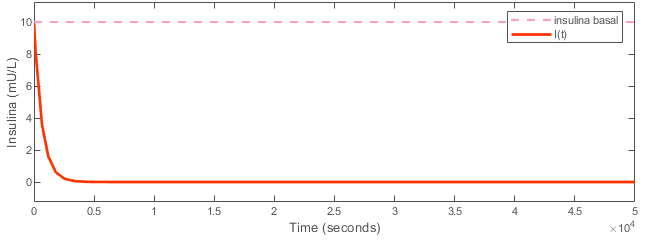
\includegraphics[width=\linewidth]{img/modelo_modificado/en_metodologia/insulina_ayuno.png}
        \caption{Insulina en ayuno diabético.}
        \label{fig:mode_ayuno_insu}
    \end{subfigure}
    
    \caption{Comportamiento de la glucosa e insulina en ayunas para un paciente diabético sin administración de insulina exógena. Fuente propia.}
    \label{fig:modificado_comportamiento_ayuno}
\end{figure}


Como se observa en las gráficas, cuando el paciente no recibe ninguna ingesta en ayuno, los niveles de glucosa en sangre se ven aumentados, pues la insulina presente en el organismo va disminuyendo (ya que hemos eliminado la insulina exógena). Los niveles de glucosa en sangre para el paciente no consiguen volver a la glucosa basal ($G_b$), pues no se está produciendo insulina en el organismo. Esta condición puede llevar a severas hiperglucemias.

\subsection{Dinámica del modelo ante una entrada: insulina exógena}

Como se ha visto anteriormente, la variable de entrada de insulina exógena U varía dependiendo del tipo de acción que induce en el organismo.
Debido a que la modelización de estos tipos de insulina y su efecto en el organismo es una labor compleja (principalmente por su variación a lo largo del tiempo), este estudio se centrará en el efecto causado por la administración de insulina en cuanto a su cantidad, y, en menor medida, respecto a su hora de administración.
1 IU de insulina humana equivale aproximadamente a 0.0347 mg. Esto se basa en la potencia biológica de la insulina, donde 1 mg de insulina tiene una actividad de aproximadamente 28.8 IU \footnote{Se establece esta relación aproximada en \cite{cima_insulina}, donde se aporta el cálculo específico para la insulina humana anhidra.}.

Para el caso basal, donde no se presentan perturbaciones externas, se espera que los niveles de glucosa e insulina permanezcan constantes en el organismo. Sin embargo, esta premisa no se cumple en sistemas glucorregulatorios alterados, los cuales exhiben una variabilidad en el nivel de glucosa basal, mostrando un aumento constante en su concentración. Se calcula, para el paciente diabético (Tabla \ref{tab:valores_diabetico}) la insulina exógena necesaria para volver a sus niveles estables de glucosa. Partiendo del estado estacionario (estudiado en la Sección \ref{sec:est_estac}), donde se ha obtenido que G(0) = Gb y que I(0)=Ib, igualamos a cero la tercera ecuación del sistema (\ref{eq:ecBergMod}), la insulina.
\begin{align}
    0= -n I(t) + \frac{U(t)}{Vi}
\end{align}
Teniendo en cuenta que I(0) = Ib:
\begin{align}
    0= -n Ib + \frac{U(t)}{Vi}
    n Ib = \frac{U(t)}{Vi}
    U(t) = n Ib Vi
\end{align}
\label{sec:insulina_calculo}
Para este paciente  se obtiene una U(t) = 0.185 mU/L. En la Figura \ref{fig:modificado_comportamiento_insulina_exogena} se muestra el efecto de la adición de esta insulina en el paciente.
\label{sec:dosis_insu_base}
\clearpage
\begin{figure}[htbp]
    \centering
    \begin{subfigure}[b]{0.9\linewidth} % Ancho ajustado al 90% del ancho de la línea
        \centering
        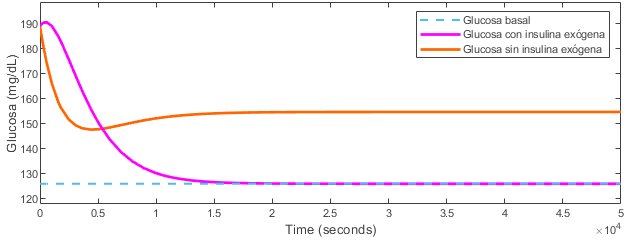
\includegraphics[width=\linewidth]{img/modelo_modificado/en_metodologia/con_insulina_glucosa.png}
        \caption{Glucosa con insulina exógena.}
        \label{fig:mod_ayuno}
    \end{subfigure}
    
    \vspace{0.5cm} % Espacio vertical entre las subfiguras

    \begin{subfigure}[b]{0.9\linewidth} % Ancho ajustado al 90% del ancho de la línea
        \centering
        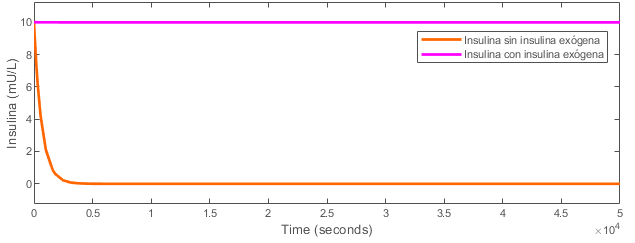
\includegraphics[width=\linewidth]{img/modelo_modificado/en_metodologia/con_insulina_insulina.png}
        \caption{Insulina con insulina exógena.}
        \label{fig:mode_ayuno_insu}
    \end{subfigure}
    
    \caption{Comparación del comportamiento de la glucosa e insulina tras una ingesta sin y con insulina exógena (U=0.185 mg). Fuente propia.}
    \label{fig:modificado_comportamiento_insulina_exogena}
\end{figure}


Se pretende abordar un segundo escenario, donde se busca encontrar el efecto en el organismo de la administración de insulina de acción rápida. Aunque esta representación puede no ser completamente precisa, se intentará diferenciar el impacto de la inyección de insulina de acción rápida en el organismo de manera tentativa, considerando su efecto inmediato en la reducción de los niveles de glucosa en sangre frente a otras formas de insulina con diferentes perfiles de acción. Para realizar esta aproximación se emplea la información relacionada con duración, pico y efecto mencionada en la Sección \ref{sec:ins_ex}, y bloques \textit{Rampa} de Simulink, cuya pendiente P se calcula:
\clearpage
\begin{small}
\begin{align}
    P ascendente = \frac{Insulina Exógena Final-Insulina Exógena Inicial}{tiempo}= \\
    \frac{Insulina Exógena Máxima-Insulina Exógena Mínima}{tiempo}\\
    P descendiente = \frac{Insulina Exógena Final-Insulina Exógena Inicial}{tiempo}=\\
    \frac{Insulina Exógena Mínima-Insulina Exógena Máxima}{tiempo}\\
\end{align}
\end{small}

\subsection{Incorporación dinámica de perturbaciones}

\subsubsection{\underline{La ingesta}}

La variable de ingesta ha sido añadida en el modelo de regulación glucémica de forma similar que en \cite{tarin2021modelo} para capturar los efectos de la alimentación en los niveles de glucosa en sangre. La ingesta D(t) se refleja en la ecuación de la glucosa G(t), presentando una relación directamente proporcional con esta, pues, a mayor cantidad de ingesta, mayores se esperan que sean los niveles de glucosa en sangre. Se modifica la ecuación de la glucosa del sistema (\ref{eq:glucosa_mod_mod}) para obtener:
\begin{align}
    \frac{dG(t)}{dt}= -p_1 (G(t) - G_b) - X(t)G(t)+D(t), G(0)=Gb \label{eq:glucosa_ingesta_bergm}
\end{align}

La ecuación particular para la ingesta, que simula un decaimiento exponencial de la ingesta una vez realizada, es denotada como D(t) y se modela de la siguiente forma:
\begin{align}
    D(t)= \frac{D_g A_g t e^{-t/t_\text{max,i}}}{V_g t^{2}_\text{max,g}} \label{eq:ecu_ingesta}
\end{align}

$D_g$ es la cantidad de carbohidratos ingeridos, y representa la cantidad aproximada de ingesta del paciente, excluyendo de esta información el valor proteico o las grasas de la comida..
Esta ecuación describe la dinámica de la ingesta a lo largo del tiempo, considerando factores como la dosis, la amplitud, el tiempo de máximo, el volumen de distribución y su variación temporal (cuyos valores se encuentran incluidos en la Tabla \ref{tab:parametros_ingesta}).

La gráfica que genera esta ecuación se encuentra en la Figura \ref{fig:grafica_ingesta} para una cantidad de 50 gramos de carbohidratos. 

\begin{table}[htbp]
    \centering
    \caption{Valores de las constantes de la función ingesta.}
    \begin{tabular}{|c|c|c|}
        \hline
          & Valor & Unidad  \\
        \hline
        Ag & 0.8 & mmol/L \\
        Tmax,i & 55 & mU/L \\
        Tmax,g & 40 & $min^-1$ \\
        Vg & 13.79 & L \\
        \hline
    \end{tabular}
    \label{tab:parametros_ingesta}
\end{table}


\begin{figure}[htbp]
    \centering
    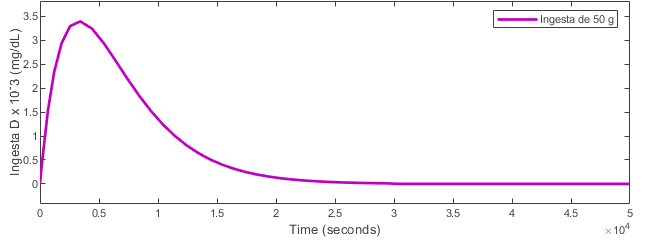
\includegraphics[width=0.9\linewidth]{img/modelo_modificado/en_metodologia/ingesta_sola.png}
    \caption{Gráfica de la ingesta D modelada según la ecuación \ref{eq:ecu_ingesta}. Fuente propia.}
    \label{fig:grafica_ingesta}
\end{figure}


\subsubsection{\underline{El ejercicio físico}}

La variable de ejercicio físico, Ej(t), ha sido incorporada en el modelo de regulación glucémica (Sección \ref{eq:glucosa_mod_mod}) para capturar los efectos de la actividad física en los niveles de glucosa en sangre. La influencia del ejercicio se refleja en la ecuación dinámica de la glucosa.  
\begin{equation} \label{eq:ejercicio_bergman}
\frac{dG(t)}{dt}= -p_1 (G(t) - G_b) - X(t)Ej(t)G(t)+D(t), G(0)=Gb 
\end{equation}
Su implementación se basa en la consideración de dos niveles de actividad física: una contribución constante durante la mayor parte del día (que representa la actividad de bajo nivel o bien la inactividad) y un período de ejercicio adicional de intensidad moderada. En los intervalos donde se produce el aumento de actividad física, se produce una contribución adicional que se suma a la contribución constante. 
La tasa de contribución constante de ejercicio al metabolismo empleada en \cite{tarin2021modelo}, es la indicada en la ecuación (\ref{eq:ejercicio_ec_bergman}) y simulada en la Figura \ref{fig:grafica_ejercicio} y se expresa en unidades de flujo por minuto. 
\begin{align} \label{eq:ejercicio_ec_bergman}
cons = 0.005/60 \\
Ej = 0.005/60 + cons,\text{si se está realizando ejercicio.}
\end{align}

\begin{figure}[htbp]
    \centering
    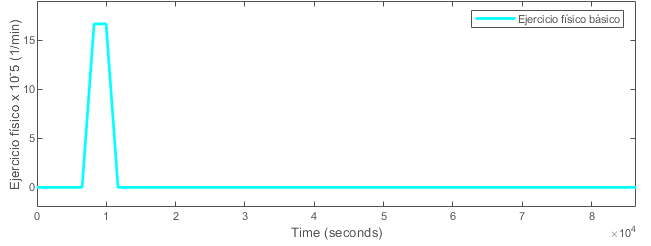
\includegraphics[width=0.9\linewidth]{img/modelo_modificado/en_metodologia/ejercicio.png}
    \caption{Gráfica de la ingesta D modelada según la ecuación \ref{eq:ejercicio_ec_bergman}. Fuente propia.}
    \label{fig:grafica_ejercicio}
\end{figure}

Se lleva a cabo una comparación entre la realización de ejercicio físico antes y después de las ingestas, basada en un estudio publicado en el American Journal of Medicine. Este estudio sugiere que la actividad física puede tener un efecto más pronunciado en la reducción de los niveles de glucosa en sangre y en la mejora de la sensibilidad a la insulina después de las comidas \footnote{Se hace referencia a este estudio específico disponible en el artículo publicado en  \cite{gwhospital_exercise_diabetes} para respaldar esta comparación.}.


\textbf{\underline{Análisis de la equivalencia funcional entre la insulina }} \\
\textbf{\underline{externa y el ejercicio}}

La actividad física regular conduce a numerosas adaptaciones en el músculo esquelético que permiten que genere ATP de manera más eficiente, siendo algunas de las adaptaciones clave una mayor absorción de glucosa y expresión de GLUT4, proteína captadora de glucosa. El entrenamiento físico aeróbico provoca la transformación del tipo de fibra muscular en un fenotipo más oxidativo y quizás más lento, y un aumento de la actividad y el contenido mitocondrial. Algunos de los efectos positivos y beneficios del ejercicio físico sobre la población diabética son la mejora de la hemoglobina glicosilada (HbA1c)\footnote{Más información en \cite{diabetes2006effects}}, reducción de la dosis diaria de insulina, mejora del perfil lipídico, disminución de retinopatías y menor incidencia de enfermedad cardiovascular. De particular importancia es la reducción de las necesidades de insulina después de realizar ejercicio. Los autores del artículo especularon que los pacientes tienden a reducir su dosis de insulina para prevenir la hipoglucemia inducida por el ejercicio. Además, el ejercicio reduce drásticamente la concentración de glucosa en sangre en un grado que depende de su intensidad, duración y el nivel concurrente de insulinemia. También aumentaría la absorción de glucosa estimulada por la insulina en el músculo, teniendo en cuenta que este efecto es mayor en el músculo entrenado que en el músculo no entrenado, lo que lleva a una reducción en el requerimiento de insulina.
Ahora bien, en el estudio \cite{salem2010exercise}, Mona A. Salem y otros demuestran que la práctica de ejercicio aeróbico moderado prolongado en pacientes diabéticos tipo 1 produce una reducción constante de la glucosa plasmática, así como la aparición de hipoglucemia si las concentraciones de glucosa antes del ejercicio son inferiores a 120 mg/dL.
En este apartado, se busca comparar la efectividad del ejercicio físico frente a la administración de insulina, así como explorar el efecto de combinar ambas intervenciones y su posible impacto en la reducción de las dosis de insulina necesarias.

\section{Control automático}

La administración de insulina exógena mediante dosis previamente estudiadas, atendiendo a los niveles basales del paciente, así como a la cantidad de ingesta que se va a producir constituye una mecánica efectiva para la estabilización de los niveles de glucosa en el organismo. Sin embargo, en ocasiones la determinación de la dosis y el momento adecuado de la administración, puede ser un desafío debido a la complejidad de las respuestas biológicas. 
Para abordar este problema, los sistemas de control automático son empleados para modelar y regular los niveles de glucosa. Uno de los enfoques ampliamente utilizados en ingeniería de control, por su efectividad y simpleza, es el regulador PID (Proporcional -Integral- Derivativo). Un controlador de este tipo se basa en el concepto de realimentación o feedback, calcula la acción de control u(t) en base al error e(t), diferencia entre el valor deseado w(t) para la variable controlada y su valor real y(t)  que se mide continuamente. Este concepto de puede observar en la Figura \ref{fig:lazo_cerrado} \footnote{Obtenida de los apuntes de la asignatura de Ingeniería de Control.}.

En el caso que nos ocupa, la referencia es el nivel concreto de glucosa en el que se quiere que esté el paciente, el error es la diferencia entre este nivel deseado y la glucosa real que tiene, y la acción de control (o variable manipulada) es la cantidad de insulina exógena que se tiene que administrar mediante la bomba de inyección.

En el caso de pacientes con diabetes tipo 1, este regulador, junto con la bomba de insulina (actuador) y el sensor de glucosa (transmisor), sustituye al comportamiento del páncreas.
\begin{figure}[htbp]
    \centering
    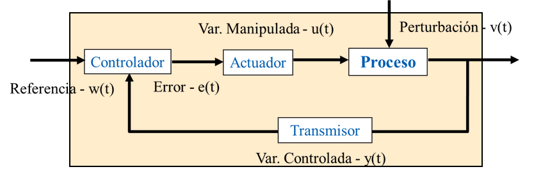
\includegraphics[width=0.9\linewidth]{img/modelo_modificado/en_metodologia/sistema en lazo cerrado.png}
    \caption{Comportamiento de un sistema en lazo cerrado. Obtenido de la asignatura de Ingeniería de Control.}
    \label{fig:lazo_cerrado}
\end{figure}

\subsection{El regulador PID}

El error, calculado como e(t) = w(t) – y(t), se incluye en la acción de control calculada de un regulador, que viene dada por la siguiente ecuación:
\begin{equation}
u(t) = Kp (e(t) + \frac{1}{Ti} \int_{0}^{t} e(\tau) \, d\tau + Td \frac{d e(t)}{dt}
\label{eq:eq_regulador}
\end{equation}
Donde se diferencian los tres términos, delimitados por signos de suma (+). Esta incluye tres parámetros fundamentales para el diseño, por orden:
\begin{enumerate}
    \item[-] Para el término proporcional, la ganancia Kp.
    \item[-] Para el término integral, el tiempo integral Ti. Ti es el tiempo que tarda la acción.
    \item[-] Para el término derivativo, el tiempo derivativo Td.
\end{enumerate}

\subsubsection{Problemática del regulador proporcional}
\label{sec:problematica_P}
Se comenzará por el regulador P, que se rige por la siguiente acción de control:
\begin{equation}
u(t) = Kp * error(t)
\label{eq:termino_P}
\end{equation}
Además, para este tipo de regulador, Kp = P (termino proporcional).

Para ciertos procesos con un regulador solo proporcional no es posible conseguir que la variable controlada alcance exactamente el valor de la referencia. Concretamente, si el error es constante, (e(t) = cte.) la acción de control u(t) es constante y no cambia más, lo que implica que la glucosa en sangre nunca se estabilice en su valor basal. E(t) se hará 0 únicamente al incluir el término integral, mediante un regulador PI.

\subsubsection{Término integral: el regulador PI}

El regulador PI adiciona a la acción de control del término proporcional P (\ref{eq:termino_P}) la siguiente acción de control:
\begin{equation}
u(t) = \frac{Kp}{Ti}\int_{0}^{t} e(\tau) \, d\tau
\label{eq:termino_I}
\end{equation}

Su relación con el término integral es: I = 1/Ti.
La idea de este tipo de regulador es calcular la acción de control u(t) de manera que si el error es constante la u(t) siga creciendo (como se observa en la ecuación (\ref{eq:termino_I})).

\subsubsection{El término derivativo D}

Debido a que un regulador P con ganancia alta para dar respuesta
rápida puede provocar oscilaciones por acción de control u excesiva, se incluye en los reguladores un nuevo término, el derivativo, cuya acción modera la u si el error decrece rápidamente, evitando estas oscilaciones. La acción derivativa se basa en la tasa de cambio del error en el tiempo, de manera que si tasa de cambio del error es alta, la acción derivativa genera una señal de control más fuerte, mientras que si la tasa de cambio es baja, la acción derivativa genera una señal más débil.

Su acción de control viene dada por la siguiente ecuación:
\begin{equation}
u(t) = Kp (e(t) + T_d \frac{d e(t)}{dt})
\label{eq:termino_d}
\end{equation}
Con esta nueva acción de control (\ref{eq:termino_d}), se consigue suavizar la respuesta de la variable controlada, pero se pueden generar cambios bruscos en la manipulada.

\subsection{Métodos de sintonía de reguladores}

El propósito de este apartado es desarrollar un modelo en Simulink que integre un regulador PID para simular el efecto de la insulina exógena en el control de los niveles de glucosa para un paciente diabético. Se emplearán métodos de sintonización sencillos para determinar los parámetros óptimos del PID.
En este contexto, se presentan dos enfoques de diseño y sintonización de reguladores. El primero es conocido como “método de prueba y error”, mientras que posteriormente se aplicará un método basado en experimentos mediante la minimización de error usando el método de López. Este método está pensado para rechazar de manera efiente las perturbaciones que afecten al proceso. En este caso, la referencia se suele mantener en el valor de la glucosa basal y lo que se pretende es mantener este nivel cuando ocurran perturbaciones como la ingesta de alimentos.

\subsubsection{Método de prueba y error}

El método basa su criterio en una estimación manual de los parámetros proporcionales e integrales del regulador. De esta forma, se parte de un valor bajo para Kp, sin acción integral ni derivativa, hasta obtener una respuesta integrada en el modelo simulado que sea similar al comportamiento de dicho modelo con una entrada de insulina exógena. Una vez realizado esto, se van modificando los valores de Ti y Td hasta lograr el comportamiento óptimo.


Se pretende demostrar, que, pese a la sencillez de implementación de este método de sintonía, la selección del valor adecuado de los parámetros es clave para el correcto funcionamiento del regulador, haciendo que una leve variación de ellos puede provocar comportamientos que supongan riesgos considerables para la estabilidad el paciente.

\subsubsection{Método basado en experimentos}

Este enfoque se basa en la realización de un experimento de salto en la entrada del sistema (en este caso, la insulina exógena) y la observación de la respuesta del sistema. Uno de los métodos ampliamente utilizados en este contexto es el Método de López, que proporciona una manera sistemática de derivar los parámetros del PID a partir de la respuesta transitoria del sistema considerando el rechazo de perturbaciones.
Este procedimiento de identificación aproxima la respuesta del proceso en lazo abierto por un sistema de primer orden con retardo, representado por la siguiente función de transferencia:
\begin{equation}
G(s) = \frac{K e^{-ds}}{\tau s +1}
\label{eq:sist_primer_o_retardo}
\end{equation}
Donde K es la ganancia, tau la constante de tiempo, y d el retardo. El cálculo de estos parámetros es necesario para la posterior obtención de los términos proporcional, integral y derivativo. Para ello, inicialmente, es necesario modelar este sistema de primer orden.
Se parte de una situación de estabilidad, en la cual, si el paciente no recibe ingestas, sus niveles de glucosa permanecen constantes gracias a la administración de insulina. Esta cantidad ha sido calculada ya en la Sección \ref{sec:dosis_insu_base}. 
A continuación, se varía el modelo para una entrada escalón de insulina, pasando de la U inicial a otra cantidad mayor de insulina. Ante esta situación, el modelo ya nos puede aportar la información necesaria para obtener los parámetros solicitados, que son:

\begin{align}
\tau = 1.5 (t2-t1) \\
d = t2- \tau \\
K= \frac{\delta y}{\delta u} \\
\label{eq:sist_primer_o_retardo}
\end{align}

Una vez obtenidos K, tau y d, se halla el valor de Kp y Ti, para lograr así obtener el valor de los términos proporcional e integral, siguiendo la misma consideración que con el método anterior, donde Kp = P, I = 1/Ti. Este cálculo se realizará mediante el método de López, que minimiza la integral del error, y es válido para procesos monótonos con d/tau <1. 
Se especifica además uno de los criterios basados en toda la respuesta, el criterio MITAE, por ser el más suavizado, cuyos valores se encuentran en las tablas \ref{tab:valores_PI_MITAE} y \ref{tab:valores_PID_MITAE}.
\begin{table}[htbp]
    \centering
    \caption{Valores de a, b para un PI con el criterio MITAE.}
    \begin{tabular}{|c|c|c|}
        \hline
        Proporcional & Integral  \\
        \hline
        a = 0.859 & a = 0.674\\
        b = -0.977 & b = -0.68\\
        \hline
    \end{tabular}
    \label{tab:valores_PI_MITAE}
\end{table}
\begin{table}[htbp]
    \centering
    \caption{Valores de a, b para un PID con el criterio MITAE.}
    \begin{tabular}{|c|c|c|}
        \hline
        Proporcional & Integral & Derivativo  \\
        \hline
        a = 1.357 & a = 0.842 & a = 0.381\\
        b = -0.947 & b = -0.738& b = -0.995\\
        \hline
    \end{tabular}
    \label{tab:valores_PID_MITAE}
\end{table}

Así, se despejan de las siguientes ecuaciones Kp y Ti:
\begin{align}
Kp K = a (\frac{d}{\tau})^b \\
\frac{\tau}{Ti} = a (\frac{d}{\tau})^b \\
\frac{Td}{\tau} = a (\frac{d}{\tau})^b \\
\label{eq:lopez}
\end{align}


\section{Técnicas y herramientas}

\subsection{MatLab}
MATLAB \cite{matlab2021matlab} es una plataforma de programación y cálculo numérico utilizada para analizar datos, desarrollar algoritmos y crear modelos. Es la abreviatura de MATrix LABoratory y ofrece un entorno de desarrollo integrado (IDE) con un lenguaje de programación propio. Se encuentra disponible para los sistemas operativos Windows, Unix, GNU/Linux y macOS. Puesto que se trata de un lenguaje con base en scripts, la creación de programas y su depuración en MATLAB con frecuencia es más fácil que en los lenguajes de programación tradicionales, como C++. MATLAB ofrece una extensa biblioteca de funciones predefinidas para realizar una variedad de tareas técnicas, siendo ampliamente empleado en campos como la ingenería.
\subsection{SIMULINK}

Simulink es una herramienta de simulación y modelado dinámico que se integra con MATLAB. Este entorno de diagramas de bloque, se utiliza para diseñar sistemas con modelos multidominio, simular antes de implementar en hardware y desplegar sin necesidad de escribir código. Simulink es particularmente útil para simular y analizar sistemas de control, sistemas de potencia, sistemas de comunicación y otros sistemas dinámicos. Además,  también ofrece capacidades de simulación avanzadas y herramientas de análisis para evaluar el rendimiento del sistema y optimizar el diseño del modelo.

\subsection{LaTex}
LaTeX \cite{latexweb} es un sistema tipográfico de alta calidad que incluye funcionalidades diseñadas para la producción de documentación técnica y científica. LaTeX es el estándar de facto para la comunicación y publicación de documentos científicos y está disponible como software gratuito. Para la realización del trabajo se emplea Overleaf, un editor LaTeX colaborativo en tiempo real, en línea y de código abierto. Para más información de este herramienta, consultar el repositorio de GitHub  \cite{overleafgithub}.



\capitulo{5}{Resultados}

Se presentan a continuación las simulaciones llevadas a cabo en este estudio.

\section{Comportamiento glucémico óptimo}
\subsection{Insulina constante y variable}

En esta sección se presentan las gráficas resultantes de la simulación de los niveles de glucosa para un paciente sano (Tabla \ref{tab:valores_no_diabetico}) usando el Modelo de Bergman con insulina constante y variable en el organismo. La suposición inicial de insulina constante es meramente hipotética (pues los niveles de glucosa no son ctes.), pero representa de forma adecuada el modelado de la glucosa para esta condición. La respuesta a la simulación tras ingesta parte de una glucosa de 135 mg/dL.
Los escenarios considerados en la Figura \ref{fig:bergman_insulinas_comp} muestran el comportamiento de la glucosa, insulina e insulina activa tras una ingesta bajo dos casos: el primero de ellos, empleando una insulina constante, donde se espera que tanto I(t) como X(t) se mantengan estables en su mismo valor (la insulina activa en 0, pues no hay variación de I(t)). Para el segundo caso, al realizar estos escenarios aplicando una insulina variable, modelada en la Ecuación (\ref{eq:insulina_variable}), se muestra un comportamiento más próximo a la realidad del sistema biológico, donde los niveles presentan algo de oscilación. Además, se observará cómo varía la insulina a lo largo del tiempo, que alcanzará un pico cuando haya mucha glucosa en el organismo, y posteriormente se estabilizará en su nivel basal. La insulina activa, por su parte, también experimentará un aumento, consecuencia del aumento de la insulina. Una vez que finalice la variación de I(t), X(t) se estabilizará de nuevo.
\clearpage

\begin{figure}[htbp]
    \centering
    \begin{subfigure}[b]{0.9\linewidth} % Ancho ajustado al 90% del ancho de la línea
        \centering
        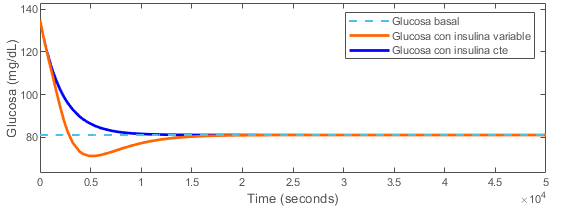
\includegraphics[width=\linewidth]{img/modelo_original/glucosa ins variable y no.png}
        \caption{Glucosa con insulina constante y variable.}
        \label{fig:bergman_glucosa}
    \end{subfigure}
    
    \vspace{0.5cm} % Espacio vertical entre las subfiguras

    \begin{subfigure}[b]{0.9\linewidth} % Ancho ajustado al 90% del ancho de la línea
        \centering
        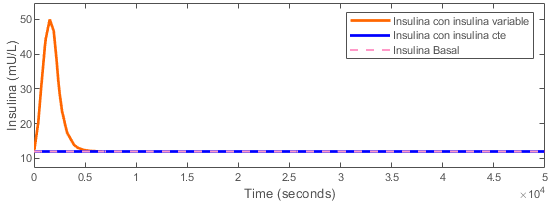
\includegraphics[width=\linewidth]{img/modelo_original/insulina ins variable y no.png}
        \caption{Insulina con insulina constante y variable.}
        \label{fig:bergman_insulina}
    \end{subfigure}

    \vspace{0.5cm} % Espacio vertical entre las subfiguras

    \begin{subfigure}[b]{0.9\linewidth} % Ancho ajustado al 90% del ancho de la línea
        \centering
        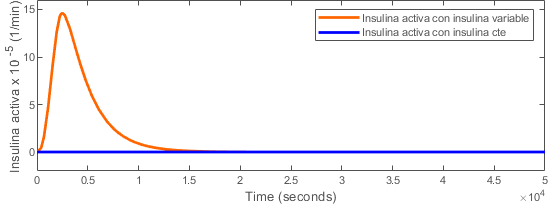
\includegraphics[width=\linewidth]{img/modelo_original/X_insvariable.png}
        \caption{Insulina activa con insulina constante y variable.}
        \label{fig:bergman_X}
    \end{subfigure}
    
    \caption{Comparativa del comportamiento de la glucosa, insulina e insulina activa tras una ingesta para una insulina constante y variable. Fuente propia.}
    \label{fig:bergman_insulinas_comp}
\end{figure}

\subsection{Variación de los parámetros del Modelo de Bergman}

Mientras que para la anterior simulación se ha seleccionado un umbral de liberación de insulina $p_5$ por parte del páncreas (Sección \ref{sec:p5})  de 90 mg/dL, se ha estudiado la \textbf{variación de este parámetro $p_5$} y su efecto en la respuesta de la glucosa. Se simulan cuatro casos, además del caso anterior ya realizado, con valores para $p_5$ de 81 mg/dL (igual que Gb), 85 mg/dL, 95 mg/dL y 100 mg/dL.
El resultado ha sido el siguiente:

\begin{figure}[htbp]
    \centering
    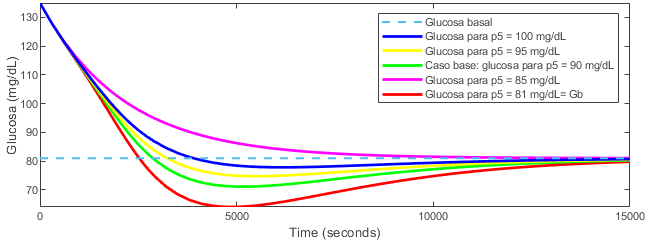
\includegraphics[width=0.9\linewidth]{img/modelo_original/p5_gluc.PNG}
    \caption{Efecto en la glucosa de la variación del umbral $p_5$. Fuente propia.}
    \label{fig:p5_gluc}
\end{figure}
\begin{figure}[htbp]
    \centering
    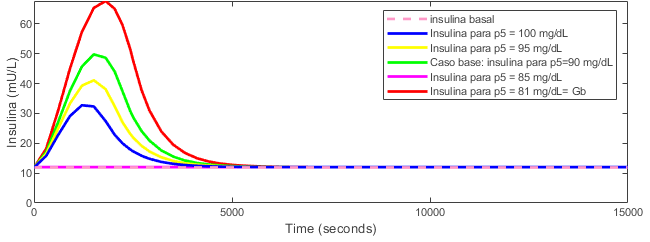
\includegraphics[width=0.9\linewidth]{img/modelo_original/p5_ins.PNG}
    \caption{Efecto en la insulina de la variación del umbral $p_5$. Fuente propia.}
    \label{fig:p5_ins}
\end{figure}

Para la glucosa, las diferencias no son muy significativas. Se observa que, de forma generalizada, que valores bajos de $p_5$ causan una menor pendiente en la estabilización de la curva de la glucosa. Aun así, la variación es escasa (pues rondan todos los supuestos valores comprendidos entre 70 y 75 mg/dL).
Para la insulina, se observa que valores más altos de $p_5$ hacen que la liberación de insulina finalice antes, pues el umbral es más alto, por lo que cuando G(t) <100, ya no se considera necesario liberar insulina. Esto hace por tanto que los niveles de insulina caigan antes a su nivel Ib. Valores más bajos de $p_5$ hacen que Ib se alcance levemente más tarde, debido a que la condición G(t) > $p_5$ sigue vigente más tiempo. El resultado es una curva cuyo tiempo de asentamiento es mayor a medida que p5 disminuye.
Valores muy bajos de p5, en este caso coincidentes con Gb (curva azul), suponen la aparición de unos niveles de insulina por debajo del basal. Tras la ingesta, y por el comportamiento variable de la insulina en el organismo, antes de estabilizarse la glucosa en su valor basal, sufre una leve disminución (ver Figura \ref{fig:p5_gluc}) inferior a Gb. Para un $p_5$ = Gb, cuando G(t)< Gb, el páncreas estima que no es necesario liberar insulina, por lo que los valores de esta caen abruptamente hasta rozar el 0.

Analizando el comportamiento del término (\ref{eq:termino_p5}) de la ecuación de la insulina (\ref{eq:insulina_variable}),

\begin{equation}
    termino = p_6 (G(t)-p_5)^+ t 
    \label{eq:termino_p5}
\end{equation}

se puede observar de manera más precisa el efecto de la variación del umbral $p_5$ en el organismo. Según lo indicado en esta ecuación (\ref{eq:termino_p5}), solo cuando la concentración de glucosa G(t) exceda el umbral $p_5$, el término completo será positivo y afectará a la insulina I(t). SI G(t) fuera menor que $p_5$, el término sería 0. Además, si G(t) > $p_5$, el término se multiplica por el tiempo, lo que sugiere un aumento de producción de insulina por el páncreas proporcional a la diferencia entre G(t) y $p_5$. Gráficamente se obtiene el mismo razonamiento en la Figura \ref{fig:termino_p5}.

\begin{figure}[htbp]
    \centering
    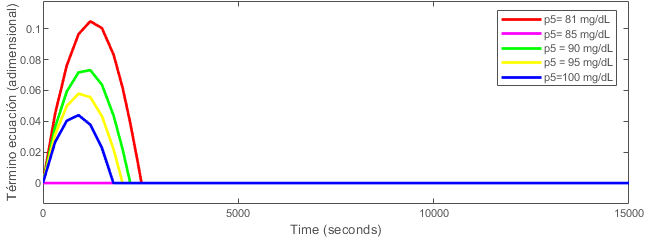
\includegraphics[width=0.9\linewidth]{img/modelo_original/p5_var/p5_termino.png}
    \caption{Comportamiento del término de la ecuación de la insulina para diferentes valores de p5. Fuente propia.}
    \label{fig:termino_p5}
\end{figure}

Acercando estas gráficas, y con la finalidad de mostrar la correlación entre este término y la glucosa respecto del tiempo, se ha calculado para la Figura \ref{fig:p5_gluc} en qué instante la glucosa G(t) para $p_5$ = 95 mg/dL alcanza dicho valor(G(t) = $p_5$ = 95 mg/dL). Se ha obtenido un tiempo t = 2030 s. Se muestra a continuación la Figura \ref{fig:zoom_p5} con el cursor establecido en este tiempo.  
\clearpage

\begin{figure}[htbp]
    \centering
    \begin{subfigure}[b]{0.9\linewidth} % Ancho ajustado al 90% del ancho de la línea
        \centering
        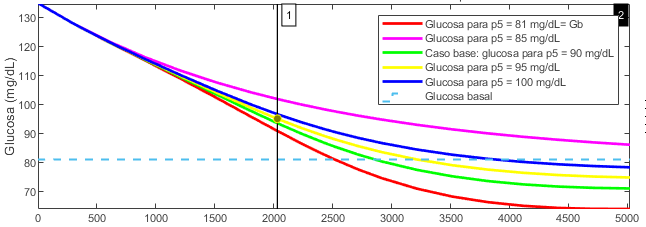
\includegraphics[width=\linewidth]{img/modelo_original/p5_var/amplio_p5_95.PNG}
        \caption{Glucosa para $p_5$.}
        \label{fig:p5_gluc_zoom}
    \end{subfigure}
    
    \vspace{0.5cm} % Espacio vertical entre las subfiguras

    \begin{subfigure}[b]{0.9\linewidth} % Ancho ajustado al 90% del ancho de la línea
        \centering
        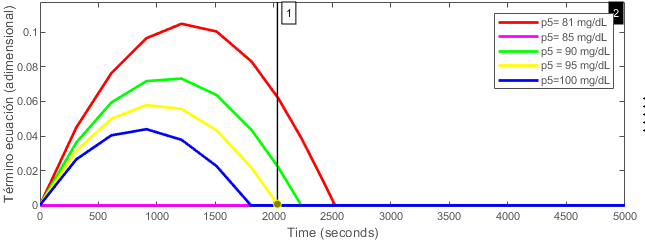
\includegraphics[width=\linewidth]{img/modelo_original/p5_var/amplio_p5_95-adi.PNG}
        \caption{Término adimensional para $p_5$.}
        \label{fig:p5_adi_zoom}
    \end{subfigure}
    
    \caption{Correlación entre la glucosa y el término adimensional de la insulina para el umbral $p_5$ en el Modelo de Bergman. Fuente propia.}
    \label{fig:zoom_p5}
\end{figure}


Se observa para la curva amarilla (correspondiente a $p_5$ =95 mg/dL) cómo en el instante en el que G(t) alcanza este valor, el término de la ecuación de la insulina se vuelve 0. Esto se debe a que la diferencia G(t) - $p_5$ se hace nula, y por tanto, su parte positiva también lo es.
Esta situación indica que, al alcanzar el valor umbral de 95 mg/dL, el estímulo para la liberación de insulina se detiene inmediatamente. En otras palabras, el páncreas deja de secretar insulina porque la concentración de glucosa ha bajado al nivel basal o por debajo de este. Este cese en la liberación de insulina no se refleja instantáneamente en la concentración de insulina I(t), ya que hay un pequeño retraso antes de que comience a disminuir, visible en la Figura \ref{fig:p5_ins}. El comportamiento aquí presente se reproduce para todos los casos simulados.

\clearpage
De la misma forma, se ha considerado realizar un pequeño análisis de los parámetros $p_1$, $p_2$ y $p_3$ del modelo. Los valores empleados se recogen en la tabla incluida en el anexo.

El efecto más significativo en la glucosa para la variación de estos parámetros se ha producido en la \textbf{tasa de eliminación de la glucosa, $p_1$}.

\begin{figure}[htbp]
    \centering
    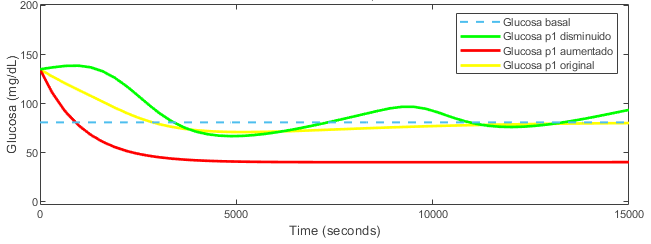
\includegraphics[width=0.9\linewidth]{img/modelo_original/p1_gl.png}
    \caption{Efecto en la glucosa de la variación de $p_1$. Fuente propia.}
    \label{fig:p1_gluc}
\end{figure}
\begin{figure}[htbp]
    \centering
    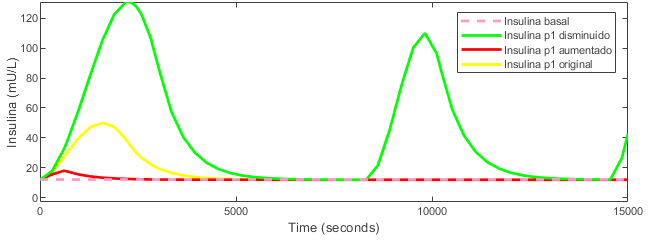
\includegraphics[width=0.9\linewidth]{img/modelo_original/p1_ins.png}
    \caption{Efecto en la glucosa de la variación de $p_1$. Fuente propia.}
    \label{fig:p1_ins}
\end{figure}

Valores \textit{aumentados de $p_1$} pueden conducir a hipoglucemia, pues al eliminarse una mayor cantidad de glucosa, sus niveles se estabilizarán por debajo de los basales, lo que representaría un importante riesgo para el paciente.  Valores \textit{disminuidos de $p_1$} conllevan a una menor velocidad de eliminación de glucosa, lo que puede resultar en oscilaciones prolongadas de los niveles de glucosa, perdiendo la capacidad para estabilizarse en un valor estacionario.
Este comportamiento se ratifica a nivel insulínico, donde valores aumentados de p1 muestran la poca necesidad de liberación de insulina por parte del páncreas, pues los niveles de glucosa son bajos. Por el contrario, valores muy disminuidos de p1 generan una respuesta anormal del organismo, no viable, donde los niveles de insulina se disparan de forma muy pronunciada. Además, no llegan a estabilizarse en un nivel basal próximo a Ib.

Los efectos de los parámetros $p_2$ y $p_3$, por ser menos significativos, se incluyen en el anexo.

\section{Comportamiento glucémico alterado}

Se muestra a continuacion el comportamiento del sistema glucorregulatorio de un \textbf{paciente diabético}. Se ha considerado llevar a cabo este análisis empleando un paciente diabético tipo 1. Su condición insulínica (de déficit absoluto), que se ha considerado “más extrema” que la presente en la diabetes tipo 2, se estima que puede reflejar mejor el comportamiento del organismo cuando la interacción glucosa – insulina se encuentra desajustada. Por tanto, se trabajará con un paciente que requiere de administración de insulina exógena (mediante el sistema de ecuaciones \ref{eq:ecBergMod} del Modelo de Bergman Modificado), pues es incapaz de producir insulina por si mismo, y, de no ser por esta administración, no podría mantener los rangos de glucosa en valores saludables. 

\subsection{Variación de la constante de tiempo n}

Como se ha indicado en la Sección \ref{sec:indicar_n}, la constante de tiempo n indica el tiempo que tarda la insulina en alcanzar el valor de la insulina exógena administrada (cte.). Pese a que para este estudio se considera el valor especificado en la Tabla \ref{tab:parametros_glucemicos}, se pretende observar si la modificación de este parámetro supone diferencias significativas en el comportamiento de la glucosa e insulina.  Se considera la insulina exógena U calculada en el apartado \ref{sec:insulina_calculo}.

Para esta simulación, se estima lo siguiente:
\begin{align}
    \text{- Si n es muy pequeño: } \frac{1}{n \downarrow} =  \uparrow \text{el tiempo para alcanzar la insulina administrada}\\
    \text{- Si n es muy grande: } \frac{1}{n \uparrow} =  \downarrow \text{el tiempo para alcanzar la insulina administrada}
\end{align}

\clearpage
\begin{figure}[htbp]
    \centering
    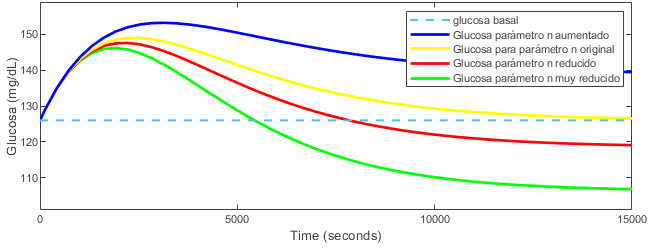
\includegraphics[width=0.9\linewidth]{img/modelo_modificado/variacion_n/n_gluco.png}
    \caption{Comportamiento de la glucosa para diferentes valores del parámetro n. Fuente propia.}
    \label{fig:n_gluc_bergm_mod}
\end{figure}
\begin{figure}[htbp]
    \centering
    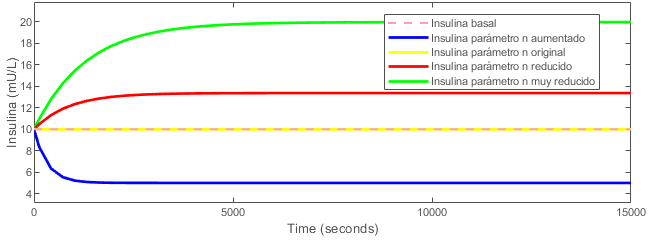
\includegraphics[width=0.9\linewidth]{img/modelo_modificado/variacion_n/n_ins.png}
    \caption{Comportamiento de la insulina para diferentes valores del parámetro n. Fuente propia.}
    \label{fig:n_ins_bergm_mod}
\end{figure}

Como se observa en las gráficas, para la insulina (Figura \ref{fig:n_ins_bergm_mod}), valores inferiores al original aumentan el tiempo que tarda la insulina en alcanzar el nivel adecuado de insulina administrada, lo que se traduce en la gráfica como una reducción de la pendiente que a su vez tarda más en estabilizarse, pues la insulina se elimina más lentamente. La mayor cantidad de insulina presente en el organismo hace que la glucosa se estabilice en un nivel más bajo que el basal. Para valores aumentados de n, la insulina se elimina más rápidamente, lo que conlleva a una disminución de la concentración de insulina en sangre. La menor cantidad de insulina disponible es menos efectiva en reducir los niveles de glucosa, lo que lleva a una estabilización en un nivel de glucosa más alto. El efecto de ello se observa en la Figura \ref{fig:n_gluc_bergm_mod} para la glucosa.


\subsection{Perturbaciones y entradas}

La ingesta se incluye en el Modelo de Bergman Modificado altamente unida al tiempo, pues delimitamos el efecto de la ingesta estableciendo un t determinado de duración de estos efectos. 
Para los ejemplos que se incluyen a continuación, se compara la ingesta de 50 y 75 gramos de carbohidratos. La gráfica de la Figura \ref{fig:ingesta_solo} muestra el comportamiento de la ingesta, y cómo, si aumentas la cantidad de carbohidratos ingeridos, la curva alcanza niveles superiores. Se observa además, que, la ingesta, una vez termina la duración del efecto, vuelve a 0, pues ya no hay resto de carbohidratos en el organismo.

\begin{figure}[htbp]
    \centering
    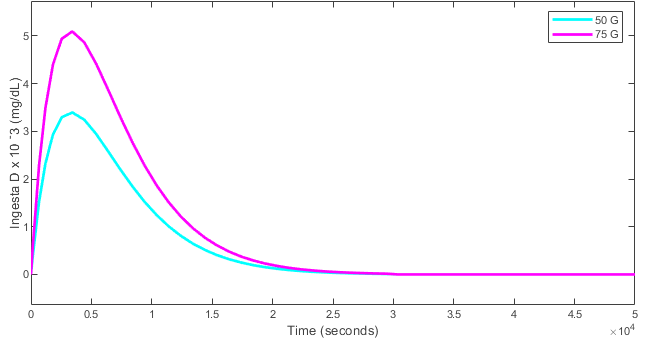
\includegraphics[width=0.9\linewidth]{img/modelo_modificado/casos base e ingesta/ingesta_sol.png}
    \caption{Curva de la función ingesta para el modelo. Fuente propia.}
    \label{fig:ingesta_solo}
\end{figure}

Para un paciente diabético, al que no le administramos insulina exógena, se obtiene un nivel en el que se estabiliza la glucosa superior a Gb (Figura \ref{fig:ingesta_glucosa}), mostrando un comportamiento incorrecto en términos regulatorios. Por tanto, si a este paciente le administramos la suficiente insulina exógena, sus niveles de glucosa volverán, tras la ingesta, a su basal Gb, así como se contribuirá a disminuir el pico máximo de glucosa.
\clearpage
\begin{figure}[htbp]
    \centering
    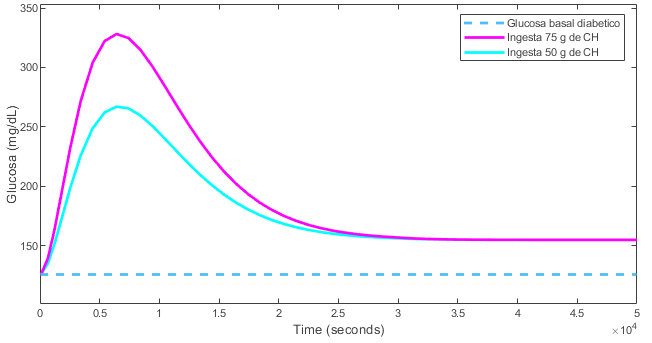
\includegraphics[width=0.9\linewidth]{img/modelo_modificado/casos base e ingesta/ing_gluc.png}
    \caption{Efecto de la ingesta en la glucosa para pacientes diabéticos. Fuente propia.}
    \label{fig:ingesta_glucosa}
\end{figure}

\underline{La insulina exógena} 

Se modela a continuación, por tanto, el comportamiento de la glucosa en sangre del paciente en ayunas considerando la insulina exógena U, como parámetro constante, reflejando, de forma relativa, el mecanismo de la insulina de acción prolongada en el organismo. 

En la Figura \ref{fig:dosis_ins} se simula el comportamiento de la glucosa y la insulina para el paciente en ayunas, bajo diferentes dosis de insulina exógena. Se observa una relación inversamente proporcional de la insulina exógena y el nivel de glucosa en sangre: cuanta más insulina externa recibe el paciente, menores serán sus niveles de glucosa en sangre. Excesos en la administración de esta insulina pueden provocar que los niveles de glucosa del paciente caigan por debajo de su nivel basal Gb, causando hipoglucemias. Por otro lado, si la insulina externa es insuficiente, los niveles de glucosa se ven aumentados llegando a causar hiperglucemias, sin alcanzar tampoco los niveles basales de glucosa. 
\clearpage
\begin{figure}[htbp]
    \centering
    \begin{subfigure}[b]{0.9\linewidth} % Ancho ajustado al 90% del ancho de la línea
        \centering
        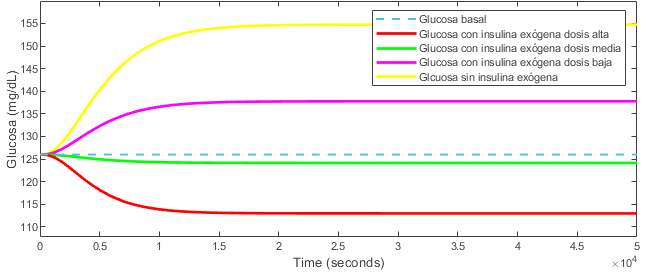
\includegraphics[width=\linewidth]{img/modelo_modificado/casos insulina/dosis_base.png}
        \caption{Glucosa con diferentes dosis de insulina exógena.}
    \end{subfigure}
    
    \vspace{0.5cm} % Espacio vertical entre las subfiguras

    \begin{subfigure}[b]{0.9\linewidth} % Ancho ajustado al 90% del ancho de la línea
        \centering
        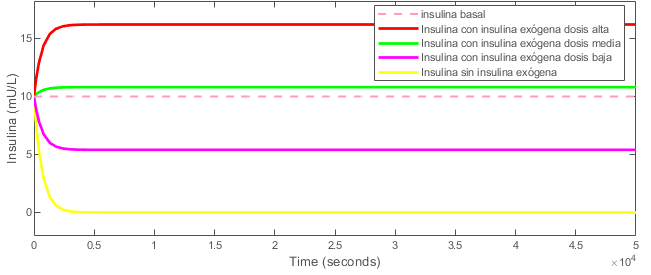
\includegraphics[width=\linewidth]{img/modelo_modificado/casos insulina/dosis_base_insul.png}
        \caption{Insulina con diferentes dosis de insulina exógena.}
    \end{subfigure}
    
    \caption{Comparativa del comportamiento de la glucosa e insulina para diferentes dosis de insulina exógena. Fuente propia.}
    \label{fig:dosis_ins}
\end{figure}


Así, administrando al paciente la dosis de insulina exógena exacta calculada para lograr que G(t)=Gb, se logra el correcto comportamiento del sistema glucorregulatorio tras la ingesta en la Figura \ref{fig:ins_ex_ing}.

Se comprueba que para este paciente, la cantidad de insulina administrada es suficiente para regular sus niveles de glucosa en sangre en ambas situaciones. Esta administración por tanto podría considerarse de insulina de acción prolongada (Sección \ref{sec:ins_prol}), donde sus efectos tienen una duración de 18-24 h, y son suficientes para estabilizar al paciente en su valor basal.
\clearpage
\begin{figure}[htbp]
    \centering
    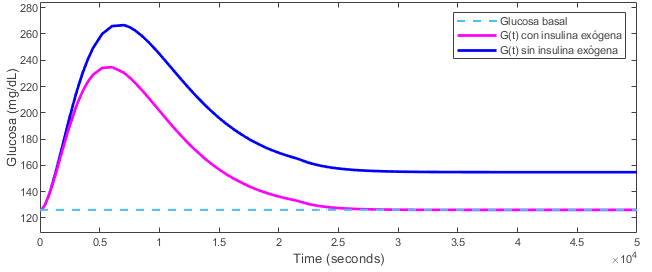
\includegraphics[width=0.9\linewidth]{img/modelo_modificado/casos insulina/ins_exacta_ing.png}
    \caption{Efecto en la glucosa de la administración adecuada de insulina externa para una ingesta. Fuente propia.}
    \label{fig:ins_ex_ing}
\end{figure}


\begin{itemize}
    \item Insulina rápida
\end{itemize}
Se ha tratado de simular el comportamiento de la insulina de acción rápida en el organismo, así como su efecto en los niveles glucémicos. Para ello se ha explorado un caso que implica la administración de insulina exógena de manera progresiva justo antes de la ingesta de alimentos. Para realizar este cálculo, se considera el tiempo necesario para que este tipo de insulina comience a actuar, el cual, como se ha indicado en la Sección \ref{sec:ins_rap}, oscila entre 5 y 20 minutos. En este contexto, se selecciona un tiempo de acción inicial de 10 minutos antes de la ingesta, alcanzando el pico de concentración de insulina administrada en 1 hora y media. Se estima que, a partir de este punto, la concentración se mantendrá constante hasta que comience a disminuir, eliminándose su efecto en un rango de 4 a 6 horas.
La ejecución de esta simulación no refleja la realidad de manera precisa, ya que este efecto “rampa” simula un comportamiento como si se administrara un porcentaje de la dosis por unidad de tiempo, aumentando progresivamente hasta alcanzar un máximo, para luego disminuir hasta llegar a cero. En la práctica clínica, el paciente se administra una inyección en un momento específico, pero para este modelo, dicho enfoque no produciría resultados significativos. A pesar de esto, el efecto de esta simulación se asemeja considerablemente al impacto que tiene la insulina rápida sobre los niveles de glucosa, justificando así la inclusión de este apartado en el estudio.
\clearpage
\begin{figure}[htbp]
    \centering
    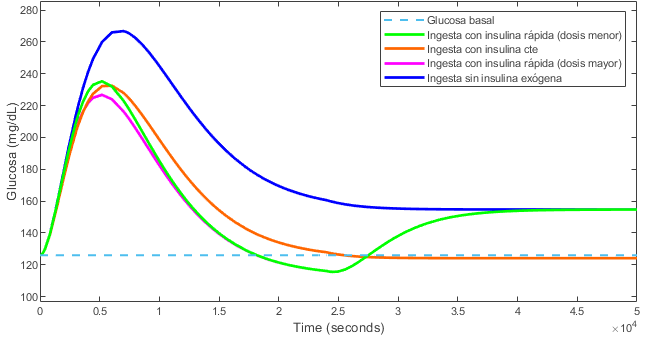
\includegraphics[width=0.9\linewidth]{img/modelo_modificado/casos insulina/caso_rapida.png}
    \caption{Efecto en la glucosa de la administración de insulina rápida y cte. Fuente propia.}
    \label{fig:ins_rap_const}
\end{figure}

Para la simulación de la insulina rápida de la Figura \ref{fig:ins_rap_const}, se observan diferencias en cuanto a la estabilización de los niveles de glucosa en el nivel basal. Para los casos de administración de insulina rápida, la glucosa logra reducir su curva considerablemente, alcanzando prácticamente los resultados de la administración de insulina cte. La pendiente de esta curva disminuye a valores inferiores a Gb, lo que indica que malas regulaciones de las dosis insulínicas puede desencadenar efectos como hipoglucemias, pese a que para este caso se encuentra dentro de límites adecuados. No se observan diferencias significativas entre las dosis de insulina rápida simuladas. Sin embargo, debido a la duración de la acción de la insulina, se observa cómo, una vez finaliza su efecto, los valores glucémicos comienzan a aumentar de nuevo, reflejando el comportamiento alterado del sistema. 

Por ello se estima simular otro caso en el que se combina la acción de la insulina rápida con la constante (Figura \ref{fig:comb_rap_cte}) con la finalidad de observar sus efectos en el sistema regulatorio.  Cabe destacar que el propósito de esta simulación es exclusivamente académico y no pretende establecer recomendaciones clínicas sobre qué tipo de insulina es mejor.
Los resultados muestran que la combinación de insulina constante con insulina rápida produce un menor pico glucémico comparado con la administración de insulina rápida por sí sola. Además, la insulina constante ayuda a estabilizar G(t) en su valor basal. Este comportamiento sugiere que la combinación de ambos tipos de insulina podría ser útil en escenarios donde la insulina prolongada por sí sola no logra reducir los picos máximos de glucosa de manera efectiva. Sin embargo, es importante resaltar que estos resultados no deben interpretarse como recomendaciones clínicas, sino como una exploración de los efectos de diferentes variables en el sistema regulatorio de la glucosa.

\begin{figure}[htbp]
    \centering
    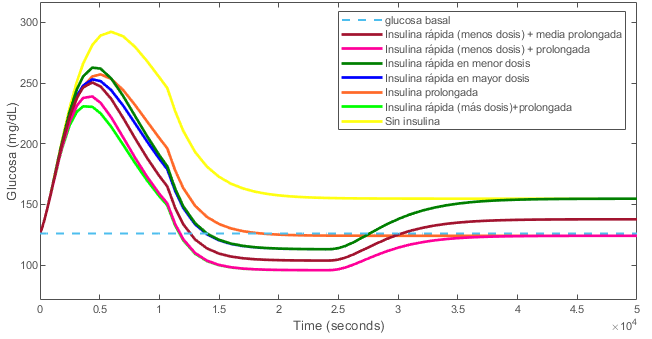
\includegraphics[width=0.9\linewidth]{img/modelo_modificado/casos insulina/combinacion.png}
    \caption{Efecto en la glucosa de la combinación en la administración de insulina rápida y cte. Fuente propia.}
    \label{fig:comb_rap_cte}
\end{figure}

\underline{El ejercicio físico} 

Se estudia el efecto en los niveles de glucosa de realizar ejercicio físico, así como la estimación del momento del día optimo para llevarlo a cabo. Se trabaja bajo la suposición de una ausencia de inyección de insulina exógena en el organismo con la finalidad de observar el efecto de la variable del ejercicio de forma aislada. La ingesta de las simulaciones contiene 50 g de carbohidratos y comienza a las 3 horas del inicio de la simulación. El ejercicio físico dura 1,2 o 3 horas, y el paciente tiene una glucosa inicial igual a su basal. Se muestran las gráficas correspondientes a la ingesta, al ejercicio y a la glucosa en sangre para el paciente.

Para los casos previos a la ingesta, estudiados en la Figura \ref{fig:ej_antes}, se observa que el efecto del ejercicio físico presenta una relación lineal, ya que a más ejercicio, menor valor de glucosa. Los casos tras ingesta de la Figura \ref{fig:ej_despues}, si que muestran relaciones diferentes entre ellos. Concretamente, cuanto antes comienza el ejercicio, más rápido disminuyen los niveles de glucosa en sangre. Además, al igual que en el caso anterior, la plena estabilización del sistema en el Gb solo ocurre para un periodo muy largo de ejercicio. 

\begin{figure}[htbp]
    \centering
    \begin{subfigure}[b]{0.9\linewidth} % Ancho ajustado al 90% del ancho de la línea
        \centering
        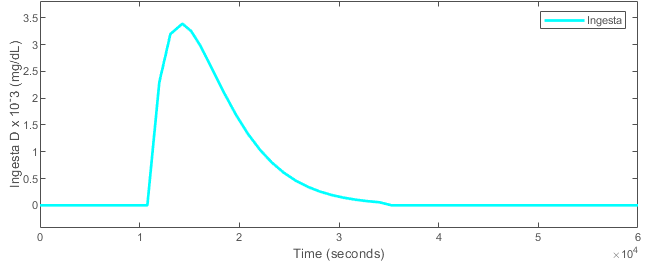
\includegraphics[width=\linewidth]{img/modelo_modificado/ejercicio/ingesta_prod.png}
        \caption{Curva de ingesta.}
    \end{subfigure}
    
    \vspace{0.5cm} % Espacio vertical entre las subfiguras

    \begin{subfigure}[b]{0.9\linewidth} % Ancho ajustado al 90% del ancho de la línea
        \centering
        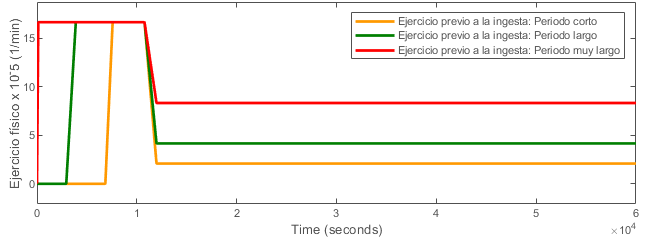
\includegraphics[width=\linewidth]{img/modelo_modificado/ejercicio/ejercicio_graf_previo.png}
        \caption{Ejercicio físico.}
    \end{subfigure}
    
    \vspace{0.5cm} % Espacio vertical entre las subfiguras

    \begin{subfigure}[b]{0.9\linewidth} % Ancho ajustado al 90% del ancho de la línea
        \centering
        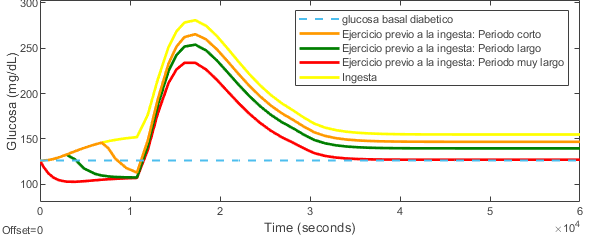
\includegraphics[width=\linewidth]{img/modelo_modificado/ejercicio/PREVIO.png}
        \caption{Curva de la glucosa.}
    \end{subfigure}
    
    \caption{Comparativa del comportamiento de la glucosa para diferentes tipos de ejercicio previos a la ingesta. Fuente propia.}
    \label{fig:ej_antes}
\end{figure}

\clearpage
\begin{figure}[htbp]
    \centering
    \begin{subfigure}[b]{0.9\linewidth} % Ancho ajustado al 90% del ancho de la línea
        \centering
        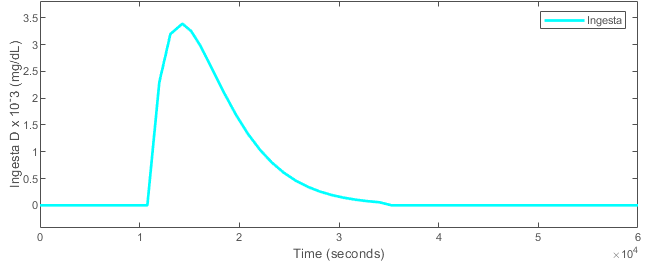
\includegraphics[width=\linewidth]{img/modelo_modificado/ejercicio/ingesta_prod.png}
        \caption{Curva de ingesta.}
    \end{subfigure}
    
    \vspace{0.5cm} % Espacio vertical entre las subfiguras

    \begin{subfigure}[b]{0.9\linewidth} % Ancho ajustado al 90% del ancho de la línea
        \centering
        \includegraphics[width=\linewidth]{img/modelo_modificado/ejercicio/ejercicio_graf_tras.png}
        \caption{Ejercicio físico.}
    \end{subfigure}
    
    \vspace{0.5cm} % Espacio vertical entre las subfiguras

    \begin{subfigure}[b]{0.9\linewidth} % Ancho ajustado al 90% del ancho de la línea
        \centering
        \includegraphics[width=\linewidth]{img/modelo_modificado/ejercicio/TRAS.png}
        \caption{Curva de la glucosa.}
    \end{subfigure}
    
    \caption{Comparativa del comportamiento de la glucosa para diferentes tipos de ejercicio tras la ingesta. Fuente propia.}
    \label{fig:ej_despues}
\end{figure}

\clearpage

\begin{itemize}
    \item Ejercicio físico e insulina
\end{itemize}

Pese a que, como se ha comprobado, la realización de ejercicio puede suponer mejoras en los niveles de glucosa, mediante los casos simulados no se logra retornar al valor basal a no ser que se aumente de forma considerable la duración del ejercicio. Se ha estimado por tanto estudiar una posible combinación entre ejercicio físico e insulina. 

Se incorpora la insulina exógena calculada anteriormente, que representa la \textit{dosis original} de insulina externa. Se estudian en este apartado diferentes proporciones de esta dosis, y se comparan con la realización de ejercicio físico. Para ello, se parte de periodos de ejercicio cortos y medios de las Figuras \ref{fig:ej_antes} y \ref{fig:ej_despues}, donde no se alcanzan los niveles basales de glucosa tras la ingesta. Es decir, la primera de las figuras compara la administración de diferentes cantidades de insulina exógena con la realización de \textbf{\textit{ejercicio corto}}, mientras que la segunda figura lleva a cabo esta comparación de dosis con el \textbf{\textit{ejercicio moderado}}.

Se observa que, para un periodo corto de ejercicio (Figura \ref{fig:ins+ej1}), no es necesaria una dosis completa de insulina. La curva morada estima que con 2/3 de la dosis original se alcanza el valor basal de glucosa, logrando estabilizarse. Para un periodo medio de ejercicio (Figura \ref{fig:ins+ej2}), la hipótesis era que se requeriría de una menor cantidad de la dosis inicial. Según las simulaciones, esta hipótesis es correcta, siendo necesaria únicamente media dosis de insulina para lograr que el paciente se estabilice en valores basales.

\begin{figure}[htbp]
    \centering
    \includegraphics[width=0.9\linewidth]{img/modelo_modificado/ejercicio/ins+ej1.png}
    \caption{Efecto en la glucosa de la combinación de un periodo corto de ejercicio físico con distintas dosis insulínicas. Fuente propia.}
    \label{fig:ins+ej1}
\end{figure}
\clearpage
\begin{figure}[htbp]
    \centering
    \includegraphics[width=0.9\linewidth]{img/modelo_modificado/ejercicio/ins+ej2.png}
    \caption{Efecto en la glucosa de la combinación de un periodo medio de ejercicio físico con distintas dosis insulínicas. Fuente propia.}
    \label{fig:ins+ej2}
\end{figure}

\section{Regulación del sistema glucosa - insulina}
\subsection{Métodos de sintonía}

Se muestran a continuación los resultados obtenidos para los dos métodos de sintonía empleados para el desarrollo del regulador: método de prueba y error, y método basado en experimentos.

\subsubsection{Método de Prueba y Error}

Para el Método de Prueba y Error, se han estimado valores para los términos proporcional e integral, concretamente, se ha desarrollado un regulador P y otro PI. En la Figura \ref{fig:prueba_error} se muestra la comparación entre ambos reguladores, así como con la administración de insulina exógena de forma manual, respecto a la ingesta sin insulina externa. 
\clearpage
\begin{figure}[htbp]
    \centering
    \begin{subfigure}[b]{0.9\linewidth} % Ancho ajustado al 90% del ancho de la línea
        \centering
        \includegraphics[width=\linewidth]{img/regulacion2/ingesta_p_e.png}
        \caption{Curva de la ingesta.}
    \end{subfigure}
    
    \vspace{0.5cm} % Espacio vertical entre las subfiguras

    \begin{subfigure}[b]{0.9\linewidth} % Ancho ajustado al 90% del ancho de la línea
        \centering
        \includegraphics[width=\linewidth]{img/regulacion2/insulina_p_e.png}
        \caption{Curva de la insulina.}
    \end{subfigure}
    
    \vspace{0.5cm} % Espacio vertical entre las subfiguras

    \begin{subfigure}[b]{0.9\linewidth} % Ancho ajustado al 90% del ancho de la línea
        \centering
        \includegraphics[width=\linewidth]{img/regulacion2/glucosa_p_e.png}
        \caption{Curva de la glucosa.}
    \end{subfigure}
    
    \caption{Gráfica de la ingesta y efecto en la insulina y la glucosa de los reguladores P y PI obtenidos mediante el Método de Prueba y Error. Fuente propia.}
    \label{fig:prueba_error}
\end{figure}

\clearpage
Como cabía esperar, tal y como se ha mencionado en la Sección \ref{sec:problematica_P} sobre la problemática del regulador proporcional, éste no es capaz de estabilizarse en valores basales, y requiere de la adición del término integral I para lograr un comportamiento adecuado. Se comprueba además que los reguladores obtenidos mediante este método de sintonía mejoran considerablemente la respuesta respecto a la administración de insulina considerada.

\begin{itemize}
    \item Variación del término P del regulador
\end{itemize}

Estudiando la variación del término proporcional en el regulador en la Figura \ref{fig:variacion_p}, cuyo ajuste óptimo es crucial para el correcto funcionamiento del sistema de regulación, se comprueba lo mencionado anteriormente. Aumentando este término respecto a su valor original, obtenemos oscilaciones en la respuesta de la glucosa, lo que puede ser perjudicial para el funcionamiento adecuado del organismo. La glucosa tiende a estabilizarse más rápidamente, pero a riesgo de presentar estas oscilaciones o sobreimpulsos debido a la respuesta más agresiva del regulador. El sistema puede volverse, así, menos estable. Por otro lado, para valores disminuidos de P, la glucosa se estabiliza más lentamente, pero la transición es más suave, con menos oscilaciones y un comportamiento más estable. Sin embargo, la gráfica de la glucosa adquiere una amplitud mucho más elevada, lo que se traduce en niveles de azúcar en sangre excesivamente altos, pudiendo causar hiperglucemias.

\begin{figure}[htbp]
    \centering
    \includegraphics[width=0.9\linewidth]{img/regulacion/variacion_p.png}
    \caption{Efecto en la glucosa de la variación del término proporcional del regulador. Fuente propia.}
    \label{fig:variacion_p}
\end{figure}



\subsubsection{Método Basado en Experimentos}

Se recogen por último los dos reguladores sintonizados mediante el método basado en experimentos, que se diferencian en la inclusión en uno de ellos del término derivativo D. La teoría dice que añadir el término derivativo anticipa la respuesta, y permite ser mas eficiente rechazando la perturbación. De hecho, con un regulador PID se disminuye el valor del pico máximo y el tiempo en volver a la referencia. 

\begin{figure}[htbp]
    \centering
    \includegraphics[width=0.9\linewidth]{img/regulacion/SINTONIZADO_PI_PID.png}
    \caption{Comparación de los reguladores sintonizados PI y PID y su efecto en la glucosa. Fuente propia.}
    \label{fig:sintonizado_PID}
\end{figure}

Se compara en la Figura \ref{fig:ejercicio_PID} el regulador PID obtenido mediante este método (en la Figura \ref{fig:sintonizado_PID}) con los casos de ejercicio físico estudiados anteriormente. Concretamente, se compara el mejor resultado de cada tipo de ejercicio (periodo muy largo, previo y tras la ingesta) con el regulador PID.

Como se puede observar, los niveles glucémicos obtenidos mediante el regulador PID son considerablemente mejores que para el resto de los casos. No solo el pico de la curva es considerablemente menor (reduciendo así el riesgo de hiperglucemias), sino que el sistema de control también permite reducir el tiempo de asentamiento de la curva, y logra estabilizarse antes en el nivel basal de glucosa.
\clearpage

\begin{figure}[htbp]
    \centering
    \begin{subfigure}[b]{0.9\linewidth} % Ancho ajustado al 90% del ancho de la línea
        \centering
        \includegraphics[width=\linewidth]{img/regulacion2/ingesta_comb.png}
        \caption{Curva de la ingesta.}
    \end{subfigure}
    
    \vspace{0.5cm} % Espacio vertical entre las subfiguras

    \begin{subfigure}[b]{0.9\linewidth} % Ancho ajustado al 90% del ancho de la línea
        \centering
        \includegraphics[width=\linewidth]{img/regulacion2/ejercicio_comb.png}
        \caption{Ejercicio físico.}
    \end{subfigure}
    
    \vspace{0.5cm} % Espacio vertical entre las subfiguras

    \begin{subfigure}[b]{0.9\linewidth} % Ancho ajustado al 90% del ancho de la línea
        \centering
        \includegraphics[width=\linewidth]{img/regulacion2/glucosa_comb.png}
        \caption{Curva de la glucosa.}
    \end{subfigure}
    
    \caption{Comparación del efecto en la glucosa del regulador PID y los mejores resultados de ejercicio físico. Fuente propia.}
    \label{fig:ejercicio_PID}
\end{figure}


Se muestra además en la Figura \ref{fig:graf_control_pid} la acción de control del regulador PID sintonizado, que se correspondería con la insulina exógena. Se comprueba cómo el regulador ejerce su efecto de control asemejándose al comportamiento de la administración de dicha insulina exógena de manera manual.
\clearpage
\begin{figure}[htbp]
    \centering
    \includegraphics[width=0.9\linewidth]{img/regulacion/control_final.png}
    \caption{Evolución de la insulina y respuesta del controlador en un sistema de infusión de insulina. Fuente propia.}
    \label{fig:graf_control_pid}
\end{figure}

En el conjunto de reguladores obtenidos se comprueba el comportamiento de la glucosa frente a estos sistemas de control, que partiendo de valores iniciales que los definen, pueden ir modelando la glucosa para adecuarla dentro de los rangos no diabéticos.
A excepción de regulador P obtenido mediante el 'Método de Prueba y Error' en la Figura \ref{fig:prueba_error}, que, como se esperaba, no logra estibilizarse en valores basales de glucosa, el resto de reguladores han logrado respuestas adecuadas. Se comprueba cómo el pico glucémico se reduce significativamente (pasando de más de 240 a valores entorno a los 180 mg/dL) para todos los casos. Los mejores resultados se obtienen con el regulador PID sintonizado, como se esperaba, pues la adición del término derivativo permite al regulador anticiparse a los cambios en el error o la señal de control, mejorando así la respuesta dinámica del sistema. 

\subsection{Comparativa paciente sano y diabético}

Por último, se incluye en la Figura \ref{fig:comparacion_diab_no_diab} la comparativa del comportamiento de la glucosa entre un paciente no diabético y un paciente diabético (cuyos valores se encuentran en la Tabla \ref{tab:valores_finales_paciente}) al que se le modela la insulina exógena con la acción de un regulador.
El regulador empleado es el PID obtenido en la sección anterior.

Para esta simulación, se trata con dos hipotéticos pacientes que cuentan con los siguientes niveles basales de glucosa e insulina:

\begin{table}[htbp]
    \centering
    \caption{Valores basales estimados para los pacientes finales.}
    \begin{tabular}{|c|c|c|}
        \hline
          & Valor\\
        \hline
        Gb & 108 mg/dL \\
        Ib & 10 mU/L  \\
        \hline
    \end{tabular}
    \label{tab:valores_finales_paciente}
\end{table}

Además, comienzan con un nivel de glucosa de 171 mg/dL (tras una ingesta).

\begin{figure}[htbp]
    \centering
    \includegraphics[width=0.9\linewidth]{img/regulacion/comparacion_no_diab.png}
    \caption{Comparación de los niveles de glucosa tras una ingesta de un paciente no diabético y un paciente diabético con regulador. Fuente propia.}
    \label{fig:comparacion_diab_no_diab}
\end{figure}

El regulador empleado sobre el paciente diabético hace que sus niveles de glucosa puedan estabilizarse en su nivel basal, de la misma forma que lo hace la administración manual de insulina exógena (incluso con mejores resultados). Para este paciente diabético, el regulador hace que la glucosa retorne a su valor basal en un tiempo de asentamiento algo menor si cabe que el propio funcionamiento del organismo del paciente no diabético. Se comprueba, por tanto, que un sistema de control en un paciente diabético permite conseguir una respuesta similar a la de un paciente sano, poniendo de manifiesto cómo es posible sustituir el comportamiento del páncreas por uno artificial.

\section{Discusión}

El modelado del sistema glucorregulatorio en el organismo llevado a cabo en este estudio ha tenido como finalidad observar el comportamiento de ciertas variables, como la glucosa e insulina, y el efecto en ellas al causar entradas y perturbaciones en el modelo, así como de los mecanismos de control.

Para un \textit{\textbf{paciente sano}}, no diabético, el comportamiento del modelo ha sido el esperado. Suponiendo inicialmente una insulina constante en el organismo, se ha mostrado cómo la glucosa mantiene constantes sus niveles en el caso de no producirse ninguna ingesta, así como los regula hasta estabilizarse en su nivel basal cuando se produce una ingesta. El modelo ha respondido bien ha esta perturbación. Sin embargo, esta hipótesis de insulina constante no se ajusta a la realidad, pues, pese a que esta variable ronda valores estables en ausencia de perturbación, el comportamiento propio del sistema no es estático, sino que es dinámico. Así, al realizar las simulaciones con la insulina variable respecto al tiempo, se observa el efecto de esta variación en las variables I(t) y X(t). Se comprueba cómo, cuando los niveles de glucosa en el organismo son elevados, se libera insulina, lo que causa un pico en la gráfica de la insulina I(t). Este cambio repercute directamente en la insulina activa, que se ve aumentada debido a la liberación de glucosa. 

Para este modelo de insulina variable se ha estudiado además el efecto de la variación del umbral del páncreas para la liberación de insulina. 
Se ha observado que valores disminuidos de $p_5$ causan una liberación más temprana de insulina ante aumentos de la glucosa, promoviendo una respuesta más rápida pero menos pronunciada en la reducción de los niveles de glucosa post-prandiales. Esta liberación de insulina lleva a la caída más temprana de sus niveles tras la ingesta, lo que podría afectar a la capacidad del organismo para mantener la glucosa en niveles normales durante peridos prolongados. Valores altos de $p_5$ se han traducido en una menor liberación de insulina, y se ha logrado una correcta estabilización de la glucosa e insulina para el paciente. Sin embargo, en casos diferentes al simulado, un aumento excesivo de este umbral puede ser perjudicial, pues el páncreas no liberará insulina hasta que los niveles de glucosa en sangre superen significativamente el umbral. Como resultado, la respuesta insulinémica se retrasará y podría ser insuficiente para manejar los aumentos moderados de glucosa después de las comidas, llegando a causar hiperglucemias.
Estos resultados subrayan la importancia crítica de calibrar correctamente el parámetro en modelos y tratamientos clínicos para garantizar una respuesta insulinémica óptima y una regulación efectiva de la glucosa.

Continuando con la importancia del ajuste de los parámetros del modelo, y teniendo en cuenta que en este estudio se ha empleado como valores originales de $p_1$, $p_2$ y $p_3$ los establecidos por Ficher en \cite{fisher1991semiclosed}, existe bastante heterogeneidad en su uso. El análisis de la variación de $p_1$, por ser el parámetro más significativo, ha estimado que un aumento en esta tasa de eliminación de glucosa puede llevar a una desestabilización del sistema por falta de glucosa en el organismo. Valores reducidos de este parámetro también causan este efecto, pero esta vez en forma de oscilaciones para la glucosa. Para la insulina, esta condición hace que se alcancen valores extremos de insulina en sangre, que son inaceptables para pacientes.

Respecto al comportamiento de la glucosa e insulina para \textit{\textbf{pacientes diabéticos}}, se ha mostrado cómo puede afectar de manera muy negativa la falta de tratamiento de la patología, resultando valores muy altos de glucosa que nunca llegan a estabilizarse. Este comportamiento se reproduce también para los casos de ingesta, pero muestra la relación contraria al incluir el ejercicio físico. Antes de hablar de esta perturbación, he considerado la administración de insulina exógena y el efecto que tiene en el organismo. Como es observable, la dosis insulínica para un paciente es única y atiende, entre otras cuestiones, a sus valores insulínicos, así como a su actividad. El ajuste adecuado de esta dosis es crucial para el tratamiento del paciente, pues de nada sirve esta administración si las dosis son excesivas, o altamente insuficientes. Cabe destacar que para este apartado la información encontrada en otras fuentes no ha sido la aquí presente, pues la insulina se incluye en la mayoría de los casos como valor constante, por lo que trato este punto como prueba experimental. En ocasiones, para los pacientes es suficiente con la insulina de acción prolongada, que mantiene su efecto durante todo el día y basta para estabilizar los niveles de glucosa en sangre. Otras veces, no es suficiente con ello, o bien se indica la administración de otro tipo de insulinas, por el efecto causado en el organismo, componentes y otras necesidades del paciente. Por ello se ha simulado también cómo sería el comportamiento de la insulina de acción rápida en el organismo, cuya implementación no está verificada pero que muestra un efecto en la glucosa acorde con el esperado. Se remarca además que no es la finalidad de este estudio proporcionar nuevas directrices o conclusiones sobre la dosificación óptima de la insulina en el organismo, sino estudiar las relaciones entre las variables y obtener comportamientos consecuentes con el sistema regulatorio. Una vez realizada esta consideración, en los resultados se puede observar que la insulina de acción rápida genera un efecto adecuado en la glucosa hasta que finaliza su dosis, donde la glucosa vuelve a sus valores atípicos. De ahí la importancia de estudiar cada caso por separado, pues, para el paciente simulado, no sería suficiente con esta insulina, ya que sus niveles de glucosa vuelven a aumentar por encima de Gb. La combinación de insulina rápida y prolongada (cte.) también se ha estudiado, de manera informativa, para comparar el efecto en los picos glucémicos de estos dos tipos de acciones. La combinación de ambas, como era esperado, es la que mejores resultados ha dado, logrando el pico menos pronunciado.
Respecto al ejercicio físico, se ha ratificado que provoca mejoras significativas en los niveles de glucosa en sangre. Aún así, es necesario recordar que esta variable se ha simulado con ecuaciones sencillas, que no representan completamente el comportamiento del organismo, sino que aportan una aproximación. Además, como se ha indicado previamente, la diabetes tipo 1 y el ejercicio pueden presentar riesgos, como la hipoglucemia. Una vez comentado este hecho, se ha estudiado el efecto generalizado del ejercicio antes y después de las comidas. Se ha seguido la hipótesis de que el ejercicio tras la ingesta era mejor que el previo a ella, y, en contra de lo esperado por mí, se ha cumplido esta hipótesis. Además, se ha cumplido la relación proporcional entre cantidad de ejercicio con mayor disminución de la glucosa. La interacción ejercicio e insulina se ha considerado para realizar una situación hipotética de combinación entre ambas variables con la finalidad de observar una reducción de los niveles de glucosa. De forma abstracta, se han considerado los casos de ejercicio moderado, que por si solos no logran retornar a los valores basales. Así, se ha determinado que para un periodo corto de tiempo de ejercicio, esta dosis sí podría verse reducida hasta en un tercio, mientras que realizando ejercicio durante un periodo medio se ha estimado una reducción de dosis mayor. Con estas demostraciones se ha pretendido verificar que las perturbaciones afectan de manera directa al sistema glucorregulatorio, de forma positiva o negativa.

Por último, en referencia a los \textit{\textbf{sistemas de control}} y mediante los métodos empleados, se comprueba que los sistemas de regulación insulínica suponen mejoras significativas, así como grandes avances en la tecnología médica. El diseño de los reguladores es un campo complejo y altamente específico en el que leves modificaciones pueden causar grandes desestabilizaciones en el sistema. Para los regulares simulados, se ha observado cómo la adición y combinación de los términos que componen el PID (Proporcional + Integral + Derivativo) causan efectos distintos. El regulador P, el más simple, aproxima su comportamiento al propio de la insulina externa en un acto de autorregulación. Un aumento de este término P disminuye el tiempo de asentamiento, es decir, disminuye el tiempo en el que la glucosa vuelve a su valor basal. Siendo este comportamiento positivo, y, pese a ello, P no logra estabilizarse en el punto basal porque el error de la acción de control nunca llega a ser cero. El regulador PI incluye un término integral que permite lograr la estabilización de G(t) y gestiona de forma adecuada el error, donde la acción de control u(t) sigue creciendo, aunque e(t) sea constante. Por otro lado, mediante métodos basados en experimentos ha sido posible sintonizar reguladores hallando el valor de sus términos mediante el método de López, mostrando otra forma de llevar a cabo este diseño. 

El comportamiento de los reguladores obtenidos presenta efectos positivos en la glucosa, a excepción del regulador P del "Método de Prueba y Error", que como se viene comentando, no llega a estabilizarse en Gb, por lo que en este caso, sería una opción descartada para el paciente. Los otros tres reguladores, destacando el regulador PID sintonizado, demuestran la capacidad del sistema de control para regular adecuadamente la curva de la glucosa, ajustando la insulina según las necesidades de la ingesta. La implementación de estos sistemas reduce considerablemente el tiempo de asentamiento de la curva, lo que supone una ventaja a la hora de evitar riesgos para el paciente. Comparando estos resultados con el comportamiento tras la ingesta de un paciente no diabético, se han logrado resultados muy similares. Este hecho sugiere que el uso de reguladores en la glucosa es altamente efectivo.
\capitulo{6}{Conclusiones}

Se recoge en este proyecto un análisis del comportamiento de la glucosa para diferentes situaciones, así como el efecto que producen en ella. 

Se ha estimado que la diabetes presenta cada vez más opciones terapéuticas de control para alcanzar la normoglucemia, y que muchas de ellas pasan por el análisis matemático de variables, cuya estimación es clave para el correcto funciomiento del sistema regulatorio aplicado. Los parámetros incluidos en estos modelos presentan valores muy específicos que han sido establecidos con el máximo rigor para evitar la aparición de riesgos en los pacientes. Se ha mostrado cómo leves variaciones en ellos pueden desembocar en fallos catastróficos en el sistema de control. Además, se ha querido mostrar la complejidad a la que tienen que hacer frente estos sistemas, que están condicionados a su vez por diversas variables que son únicas y diferentes para cada paciente. Se ha pretendido estudiar también el efecto de la combinación de diferentes opciones, entre las que ha destacado la efectividad del deporte, especialmente después de las comidas, logrando una hipotética disminución hasta en 2/3 de la dosis de insulina administrada, pese a que su marco debe ser regulado para cada paciente debido al riesgo de hipoglucemias. La combinación de diferentes acciones de insulina se ha llevado a cabo como simulaciones experimentales, con el fin de comprobar si sería posible reducir ciertas dosis de insulina prolongada si se combina con insulina rápida, cuyos resultados han sido favorables. Estos resultados son solo hipótesis, y se pretende reivindicar desde esta sección la importancia de la personalización de los tratamientos. Sin embargo, la terapia insulínica, que ha sido presentada de unos años a la actualidad como la solución más efectiva y eficaz a esta patología, comienza a verse desplazada y sustituida por grandes dispositivos de control que manejan de forma automática las descompensaciones de glucosa y administran la insulina necesaria. El efecto que esta acción produce se ha tratado de reflejar en los reguladores sintonizados, que, aunque de manera muy simple, se ha logrado la estabilización de la glucosa en su valor basal, así como la disminución de la amplitud de la curva y del tiempo de asentamiento. 
Así, la creación de grandes dispositivos de control, como el páncreas artificial, regidos por sistemas regulatorios y estimaciones matemáticas, auguran mejoras significativas para el tratamiento de la diabetes, así como en la calidad de vida para los pacientes.


\section{Aspectos relevantes}

Respecto a los aspectos más relevantes del proyecto, se pueden resumir en los siguientes puntos:
\begin{enumerate}
    \item El interés de este proyecto radica, a mi parecer, en la combinación de estrategias de ingeniería con conocimiento biológico para el desarrollo de nuevas estrategias que permitan avanzar en la diabetes. La finalidad de este proyecto no ha sido observar la variación de la glucosa a nivel biológico, sino de entender que su comportamiento puede ser regido por relaciones matemáticas que tratan de aproximarse lo máximo posible a la realidad, y que a su vez pueden ser empleadas para la obtención de soluciones médicas.
    Se trata este proyecto como el inicio del estudio del sistema glucorregulatorio para futuros estudiantes que partan de estos resultados para obtener otros nuevos. Especial relevancia adquiere para mí la modelización que se ha llevado a cabo en otros artículos mencionados a lo largo de esta memoria de funciones como la ingesta, o el ejercicio físico, cuyo comportamiento se ha estimado de manera matemática para permitir observar su efecto en la glucosa. 
    Sin embargo, a nivel insulínico, he encontrado este tema complejo, pues mediante las ecuaciones diferenciales aplicadas que simplifican profundamente el comportamiento del sistema, no se logra modelar de forma óptima algunos casos, o bien el comportamiento de la glucosa no se ajusta del todo a la realidad.
    Especial sorpresa ha tenido para mi encontrarme con una simple ecuación que represente el comportamiento del páncreas, aunque sea de forma aproximada, dándome a entender que este campo es verdaderamente complejo y busca relaciones matemáticas muy precisas.
    \item Inicialmente se estudiaron los modelos matemáticos clásicos de la glucosa, y tras una búsqueda exhaustiva, se determinó trabajar con los Modelos De Bergman y Ackerman. Tras unas pruebas iniciales mediante la inclusión de variables y pruebas de datos diferentes, se determinó que la mejor opción era el Modelo de Bergman, pues presentaba más información y ampliaciones. El Modelo de Ackerman presentó al inicio resultados confusos para variables como el ejercicio, por lo que se decidió desestimarlo para estos casos. De esta manera, se decidió emplear únicamente el Modelo de Bergman, pues para casos iniciales, sería redundante presentar el mismo comportamiento de la glucosa siguiendo dos modelos diferentes. El acceso a los modelos matemáticos de la glucosa ha resultado ser bastante restringido, lo que en ocasiones ha limitado el estudio.
    \item Una vez seleccionado el Modelo, se comenzó con el análisis de parámetros y de su comportamiento. Pese a la definición de las ecuaciones por Bergman en \cite{bergman1979quantitative}, se han encontrado complicaciones a nivel matemático, pues, desde entonces, el Modelo ha avanzado mucho, como en el propuesto en \cite{fisher1991semiclosed}, donde no se termina de aclarar el procedimiento matemático seguido. Además, el valor de los parámetros del modelo se ha establecido que fueran los seleccionados en el artículo anteriormente mencionado, lo que invita a pensar que tienen un carácter general y que no son personalizados para cada paciente, de ahí el análisis realizado en este estudio sobre ellos.
    \item En cuanto a la administración de insulina exógena, se ha realizado un apartado estudiando la combinación de diferentes estrategias para pacientes diabéticos. Pese a que se ha tratado solo de un marco hipotético, me ha resultado sorprendente visualizar el efecto de los tipos de insulinas según su forma de acción, mostrando cómo la administración de insulina constante (a la que se ha considerado insulina prolongada), causa una reducción general de los niveles de glucosa en el organismo; mientras que la insulina de acción rápida ejerce un efecto más significativo pero en menores intervalos de tiempo. Sin embargo, este apartado se ha visto condicionado por la poca distinción entre tipos de insulina externa que he encontrado en refeencia a modelos matemáticos. Cabe remarcar que para este apartado se ha reflejado \textit{el efecto} de estas combinaciones en la glucosa, pero su modelado no se corresponde con la realidad. Para el caso de la insulina prolongada, se ha determinado una insulina constante para todo el día, comportamiento que no es del todo cierto, puesto que, pese a que este tipo de insulina presenta una duración de acción de 18 - 24 h, no supone una administración constante de insulina. Por otro lado, la insulina de acción rápida se ha modelado como una rampa, donde se ha calculado la pendiente de la curva de la insulina para lograr en el tiempo de pico de acción el nivel máximo, mientras que luego esos niveles se van reduciendo hasta desaparecer (siguiendo la duración de esta insulina en el organismo). Este comportamiento en la realidad se correspondería con un paciente al que se le está administrando la insulina de manera continua y progresiva en vez de con una dosis puntual. Sin embargo, el efecto en la glucosa si que se ha considerado el deseado.
    \item Respecto a la combinación de estrategias, se ha realizado también de manera hipotética un experimento con el fin de comparar la administración de una dosis mayor de insulina prolongada y la administración de esta insulina en menor dosis, combinada con el ejercicio y la insulina rápida. La finalidad de esta simulación ha sido determinar que existen factores que dependen del paciente, como el deporte, que sí que pueden contribuir a reducir los niveles de glucosa, disminuyendo la necesidad de alternativas de administración de insulina. Lejos de desprestigiar las dosis insulínicas, se pretende con este apartado mostrar las alternativas y el efecto de diferentes combinaciones en el organismo.
    \item Mediante los sistemas de control estudiados y sintonizados se ha comprobado su eficacia, y la extensión de esta eficacia a grandes dispositivos que facilitan la calidad de vida de muchos pacientes. Llamativa ha sido la comparación de los reguladores obtenidos con el mecanismo de una persona sana, dando a entender que el comportamiento de la glucosa varía para cada individuo y que se pueden conseguir tan buenos resultados a nivel glucorregulatorio como los que se obtienen con un sistema no alterado.
    \item Por último, respecto al testeado del modelo con datos reales, hubo una puesta en contacto personal con el Servicio de Nutrición del Hospital de Burgos (HUBU) para la solicitud de informes diabéticos, pero tras redactar el Informe de la Comisión de Bioética, no se logró realizar un acuerdo.
\end{enumerate}



\capitulo{7}{Lineas de trabajo futuras}



Como líneas futuras de este proyecto se proponen las siguientes:
\begin{enumerate}
    \item [-] En primer lugar, el empleo de este estudio como base para aplicar modelados matemáticos más complejos u otros no mencionados como el de Jonh Sorensen, modelos que incluyan el retraso, o el Simulador Metabólico de Diabetes tipo 1(T1DMS), o bien modelos novedosos por desarrollar. Estos modelos podrían proporcionar una comprensión más completa de la fisiopatología de la diabetes y permitir la simulación de diferentes escenarios clínicos y tratamientos.
    \item[-] Continuar con el estudio de los mecanismos de control de la glucosa a partir del algorimto de control clásico PID propuesto, explorando enfoques más sofisticados y precisos. Esto podría llevarse a cabo bien analizando reguladores ya creados o bien desarrollando unos nuevos, adaptándose mejor a la naturaleza dinámica y no lineal (como se ha considerado en alguna ocasión para este estudio) del sistema glucorregulatorio. En este apartado se encontraría incluso el desarrollo de glucómetros que permita la lectura de valores de glucosa muy elevados (pues en muchos de ellos, cuando el sensor detecta un límite máximo determinado,deja de captar niveles de concentración superiores). Entre los sistemas que propongo se encuentran los reguladores de control predictivo (que preveen el comportamiento futuro de la glucosa y calcula la señal de control a partir de funciones de costo predefinidas), los de control adaptativo (que ajustan los parámetros en función de las condiciones del sistema de forma continua), o el regulador feedfordward, que se anticipa y compensa las perturbaciones antes de que afecten al sistema (a los niveles de glucosa, en este caso). A diferencia de los anteriores, este regulador no actúa en respuesta a una señal de error, sino que ajusta la señal de manera proactiva. 
    \item [-] Estudiar de manera más detallada y realista el modelado de los diferentes tipos de insulina exógena, considerando su cinética de absorción y acción, analizando cómo se liberan en el torrente sanguíneo y cómo es posible modelar estas relaciones. Esto mejoraría la personalización del tratamiento insulinoterapéutico, así como contribuiría a una optimización de las estrategias de dosificación de la insulina.
    \item[-] Abordar el efecto de otras variables de interés en la interacción de la glucosa e insulina, como el estrés, la calidad del sueño, o la ansiedad, y tratar de obtener relaciones entre ellas. Respecto a la más interesante para mí, el estrés, se conoce que la liberación del cortisol y adrenalina aumenta los niveles de glucosa en sangre al promover la liberación de la glucosa almacenada en el hígado y al reducir la sensibilidad a la insulina. El estrés crónico aumenta el riesgo a desarrollar Diabetes Tipo 2, y puede incluso causar el agotamiento de las células beta del páncreas.
    \item[-] Combinar el modelado matemático llevado a cabo con nuevas tecnologías y enfoques, para mejorar el monitoreo de la diabetes, así como unir este campo con la inteligencia artificial. Este análisis podría servir de base para la introducción a la ingeniería de tejidos pancreáticos o las terapias con células beta.
\end{enumerate}


\bibliographystyle{apalike}
\bibliography{bibliografia}

\end{document}